%%%%%%%%%%%%%%%%%%%%%%%%%%%%%%%%%%%%%%%%%
% Masters/Doctoral Thesis 
% LaTeX Template
% Version 1.41 (9/9/13)
%
% This template has been downloaded from:
% http://www.latextemplates.com
%
% Original authors:
% Steven Gunn 
% http://users.ecs.soton.ac.uk/srg/softwaretools/document/templates/
% and
% Sunil Patel
% http://www.sunilpatel.co.uk/thesis-template/
%
% License:
% CC BY-NC-SA 3.0 (http://creativecommons.org/licenses/by-nc-sa/3.0/)
%
% Note:
% Make sure to edit document variables in the Thesis.cls file
%
%%%%%%%%%%%%%%%%%%%%%%%%%%%%%%%%%%%%%%%%%

%----------------------------------------------------------------------------------------
%	PACKAGES AND OTHER DOCUMENT CONFIGURATIONS
%----------------------------------------------------------------------------------------

\documentclass[11pt, a4paper, oneside]{Thesis} % Paper size, default font size and one-sided paper
% \documentclass{Thesis}
\graphicspath{{Pictures/}} % Specifies the directory where pictures are stored

\usepackage{float}[2001/11/08]%    v1.3d
\usepackage{placeins}[2005/04/18]% v2.2  ; for \FloatBarrier
\usepackage{rotating}[2009/03/28]% v2.16a; for sidewaystable-environment
\usepackage{hyperref}[2012/11/06]% v6.83m

% \usepackage{tablefootnote}[2014/01/26]%   v1.1c
\usepackage[square, comma, sort&compress]{natbib} % Use the natbib reference package - read up on this to edit the reference style; if you want text (e.g. Smith et al., 2012) for the in-text references (instead of numbers), remove 'numbers' 
\hypersetup{urlcolor=blue, colorlinks=true} % Colors hyperlinks in blue - change to black if annoying
\title{\ttitle} % Defines the thesis title - don't touch this

\begin{document}

\frontmatter % Use roman page numbering style (i, ii, iii, iv...) for the pre-content pages

\setstretch{1.3} % Line spacing of 1.3

% Define the page headers using the FancyHdr package and set up for one-sided printing
\fancyhead{} % Clears all page headers and footers
\cfoot{\thepage} % Sets the right side header to show the page number
% \lhead{} % Clears the left side page header

\pagestyle{fancy} % Finally, use the "fancy" page style to implement the FancyHdr headers

\newcommand{\HRule}{\rule{\linewidth}{0.5mm}} % New command to make the lines in the title page

% PDF meta-data
\hypersetup{pdftitle={\ttitle}}
\hypersetup{pdfsubject=\subjectname}
\hypersetup{pdfauthor=\authornames}
\hypersetup{pdfkeywords=\keywordnames}

%----------------------------------------------------------------------------------------
%	TITLE PAGE
%----------------------------------------------------------------------------------------

% \begin{titlepage}
\pagestyle{empty}
\begin{center}

\vspace*{6ex}
{\huge \bfseries Implementing and Accelerating\\ HMMER3 Protein Sequence Search on CUDA-Enabled GPU}\\[4cm] % Thesis title
 
\textsc {\Large \href{http://ca.linkedin.com/pub/lin-cheng/19/191/422} \authornames}\\[3cm] % Thesis type

\large \textsc{A thesis\\ in\\ The Department\\ of\\ \deptname }\\[3cm] % University requirement text
{Presented in Partial Fulfilment of the Requirements\\ For the Degree of \degreename \\ \univname\\ Montr\'{e}al, Qu\'{e}bec, Canada}\\[1cm]
 
{\large \today}\\ % Date
{\textcopyright \authornames, 2014}
%\includegraphics{Logo} % University/department logo - uncomment to place it
 
\vfill
\end{center}

% \end{titlepage}

\clearpage

\pagestyle{empty} % No headers or footers for the following pages
  \vspace{1em}
%     \vspace{1ex}
     \begin{center}
        CONCORDIA UNIVERSITY
     \end{center}
     \begin{center}
        School of Graduate Studies
     \end{center}
     \vspace{3ex}
     This is to certify that the thesis prepared\\[2ex]
     By :\hspace{38pt}{\bf {\authornames}}\\[2ex]
     Entitled :\hspace*{13pt}{\bf \ttitle}\\[2ex] 
    and submitted in partial fulfilment of the requirements for the degree
    of\\[2ex]
    \hspace*{62pt}{\bf \degreename}\\[2ex]
    complies with the regulations of this University and meets the accepted
    standards with respect to originality and quality. \\[2ex]
    Signed by the final examining committee : \\[5ex]
    \hspace*{77pt}\underline{\hspace{234pt}} Chair\\
    \hspace*{77pt}Dr.\@ Brigitte Jaumard \\[2.5ex]
    \hspace*{77pt}\underline{\hspace{234pt}} Examiner\\
    \hspace*{77pt}Dr.\@ Dhrubajyoti Goswami \\[2.5ex]
    \hspace*{77pt}\underline{\hspace{234pt}} Examiner\\
    \hspace*{77pt}Dr.\@ Hovhannes A. Harutyunyan \\[2.5ex]
    \hspace*{77pt}\underline{\hspace{234pt}} Supervisor \\
    \hspace*{77pt}\@ \supname\\[2.5ex]
    Approved by \hspace{9pt}\underline{\hspace{232pt}}\\
    \hspace*{79pt}Chair of Department or Graduate Program Director\\[6ex]
    \underline{\hspace*{100pt}} \hspace{10pt}  2014. \hspace{48pt} \underline{\hspace{200pt}}\\
    \hspace*{200pt}Dr.\@ Robin A. L. Drew \\
    \hspace*{200pt}Dean of Faculty\\    
    \hspace*{200pt}(\deptname)

\clearpage

%----------------------------------------------------------------------------------------
%	ABSTRACT PAGE
%----------------------------------------------------------------------------------------

% \addtotoc{Abstract} % Add the "Abstract" page entry to the Contents

%   \thispagestyle{empty}
%   \null\vfil
%   \begin{center}
%     \setlength{\parskip}{0pt}
%     \bigskip
%     {\huge{\textit{Abstract}} \par}
%     \bigskip
%     \bigskip
%     {\normalsize\bf \@title \par} % Thesis title
%     \medskip
%     {\normalsize \authornames \par} % Author name
%     \bigskip
%   \end{center}
\pagestyle{fancy}
\abstract{{\vspace{1em}} % Add a gap in the Contents, for aesthetics

The recent emergence of multicore CPU and manycore GPU architectures has made parallel computing more accessible. Hundreds of industrial and research applications have been mapped onto GPUs to further utilize the extra computing resource.
In bioinformatics, HMMER is a set of widely used applications for sequence analysis based on Hidden Markov Model. One of the tools in HMMER, \emph{hmmsearch}, and the Smith-Waterman algorithm are two important tools for protein sequence analysis that use dynamic programming. Both tools are particularly well-suited for many-core GPU architecture due to the parallel nature of sequence database searches. 

After studying the existing research on CUDA acceleration in bioinformatics, this thesis investigated the acceleration of the key Multiple Segment Viterbi algorithm in HMMER version 3. A fully-featured CUDA-enabled protein database search tool \emph{cudaHmmsearch} was designed, implemented and optimized. We demonstrated a variety of optimization strategies that are useful for general purpose GPU-based applications. Based on our optimization experience in parallel computing, six steps were summarized for optimizing performance using CUDA programming. 

We made comprehensive tests and analysis for multiple enhancements in our GPU kernels in order to demonstrate the effectiveness of selected approaches. The performance analysis showed that GPUs are able to deal with intensive computations, but are very sensitive to random accesses to the global memory. The results show that our implementation achieved 2.5x speedup over the single-threaded HMMER3 CPU SSE2 implementation on average.

}
\clearpage % Start a new page

%----------------------------------------------------------------------------------------
%	ACKNOWLEDGEMENTS
%----------------------------------------------------------------------------------------

\setstretch{1.3} % Reset the line-spacing to 1.3 for body text (if it has changed)

% \acknowledgements{\addtocontents{toc}{\vspace{1em}} % Add a gap in the Contents, for aesthetics
\acknowledgements{{\vspace{1em}} % Add a gap in the Contents, for aesthetics

First, I am truely thankful to my supervisor {\supname} for his profound knowledge, flexibility in supervising students, warm-hearted, and selecting this interesting topic for my research.

I also give thanks to my friendly group: Faizah Aplop, Christine Houry Kehyayan, Nada Alhirabi, Asma Mistadi and Qing Ye for their communicating and helping me know more about Bioinformatics and life in Montreal, Stuart Thiel for providing Kronos machine as my developing and benchmarking environment.

My deepest gratitude goes to my family in China for their unquestioning love. I miss them so much in Canada. Hope less visa trouble between the two countries I love.

}
\clearpage % Start a new page

%----------------------------------------------------------------------------------------
%	LIST OF CONTENTS/FIGURES/TABLES PAGES
%----------------------------------------------------------------------------------------

\thispagestyle{plain} % The page style headers have been "empty" all this time, now use the "fancy" headers as defined before to bring them back

% \lhead{\emph{Contents}} % Set the left side page header to "Contents"
\tableofcontents % Write out the Table of Contents

% \lhead{\emph{List of Figures}} % Set the left side page header to "List of Figures"
\listoffigures % Write out the List of Figures

\lhead{\emph{List of Tables}} % Set the left side page header to "List of Tables"
\listoftables % Write out the List of Tables

%----------------------------------------------------------------------------------------
%	ABBREVIATIONS
%----------------------------------------------------------------------------------------

\clearpage % Start a new page

\setstretch{1.5} % Set the line spacing to 1.5, this makes the following tables easier to read

\lhead{\emph{Abbreviations}} % Set the left side page header to "Abbreviations"
\listofsymbols{ll} % Include a list of Abbreviations (a table of two columns)
{
\textbf{CUDA} & \textbf{C}ompute \textbf{U}nified \textbf{D}evice \textbf{A}rchitecture \\
\textbf{DMA} & \textbf{D}irect \textbf{M}emory \textbf{A}ccess \\
\textbf{DP} & \textbf{D}ynamic \textbf{P}rogramming \\
\textbf{GPU} & \textbf{G}raphics \textbf{P}rocessing \textbf{U}nit \\
\textbf{HMM} & \textbf{H}idden \textbf{M}arkov \textbf{M}odel \\
\textbf{HMMER} & \textbf{H}idden \textbf{M}arkov \textbf{M}odel\textbf{ER} \\
\textbf{MPI} & \textbf{M}essage \textbf{P}assing \textbf{I}nterface \\
\textbf{MSV} & \textbf{M}ultiple \textbf{S}egment \textbf{V}iterbi \\
\textbf{NCBI} & \textbf{N}ational \textbf{C}enter for \textbf{B}iotechnology \textbf{I}nformation) \\
\textbf{NR} & \textbf{N}on-\textbf{R}edundant \\
\textbf{OS} & \textbf{O}perating \textbf{S}ystem \\
\textbf{Pfam} & \textbf{P}rotein \textbf{fam}ilies \\
\textbf{SIMD} & \textbf{S}ingle-\textbf{I}nstruction \textbf{M}ultiple-\textbf{D}ata \\
\textbf{SM} & \textbf{S}treaming \textbf{M}ultiprocessors \\
\textbf{SSE} & \textbf{S}treaming \textbf{S}IMD \textbf{E}xtensions \\
\textbf{SW} & \textbf{S}mith-\textbf{W}aterman
% \textbf{LAH} & \textbf{L}ist \textbf{A}bbreviations \textbf{H}ere \\
% \textbf{Acronym} & \textbf{W}hat (it) \textbf{S}tands \textbf{F}or \\
}

%----------------------------------------------------------------------------------------
%	PHYSICAL CONSTANTS/OTHER DEFINITIONS
%----------------------------------------------------------------------------------------

% \clearpage % Start a new page
% 
% \lhead{\emph{Physical Constants}} % Set the left side page header to "Physical Constants"
% 
% \listofconstants{lrcl} % Include a list of Physical Constants (a four column table)
% {
% Speed of Light & $c$ & $=$ & $2.997\ 924\ 58\times10^{8}\ \mbox{ms}^{-\mbox{s}}$ (exact)\\
% % Constant Name & Symbol & = & Constant Value (with units) \\
% }

%----------------------------------------------------------------------------------------
%	SYMBOLS
%----------------------------------------------------------------------------------------

% \clearpage % Start a new page
% 
% \lhead{\emph{Symbols}} % Set the left side page header to "Symbols"
% 
% \listofnomenclature{lll} % Include a list of Symbols (a three column table)
% {
% $a$ & distance & m \\
% $P$ & power & W (Js$^{-1}$) \\
% % Symbol & Name & Unit \\
% 
% & & \\ % Gap to separate the Roman symbols from the Greek
% 
% $\omega$ & angular frequency & rads$^{-1}$ \\
% % Symbol & Name & Unit \\
% }

%----------------------------------------------------------------------------------------
%	DEDICATION
%----------------------------------------------------------------------------------------

% \setstretch{1.3} % Return the line spacing back to 1.3
% 
% \pagestyle{empty} % Page style needs to be empty for this page
% 
% \dedicatory{For/Dedicated to/To my\ldots} % Dedication text
% 
% \addtocontents{toc}{\vspace{2em}} % Add a gap in the Contents, for aesthetics

%----------------------------------------------------------------------------------------
%	THESIS CONTENT - CHAPTERS
%----------------------------------------------------------------------------------------

\mainmatter % Begin numeric (1,2,3...) page numbering

\pagestyle{fancy} % Return the page headers back to the "fancy" style
\pagestyle{plain}
% Include the chapters of the thesis as separate files from the Chapters folder
% Uncomment the lines as you write the chapters

% Chapter Template

\chapter{Introduction} % Main chapter title

% \label{Intro} % Change X to a consecutive number; for referencing this chapter elsewhere, use \ref{ChapterX}

\lhead{Chapter 1. \emph{Introduction}} % Change X to a consecutive number; this is for the header on each page - perhaps a shortened title

%----------------------------------------------------------------------------------------
%	SECTION 1
%----------------------------------------------------------------------------------------
\section{Problem Statement}
What's it + why important

History of problem + state of art

Summary of work + contribution

Discuss common use of HMMER

HMMER \citep{HMMER} is a free and commonly used software package for sequence analysis written by Sean Eddy. 
It is an open source implementation of HMM algorithms for use with protein databases.

One of its more widely used applications, \emph{hmmsearch} is to identify homologous protein. It does this with Viterbi algorithm by comparing a profile HMM to each protein sequence in a large database, evaluating the path that has the maximum probability of the HMM generating the sequence.
This search requires a computationally intensive procedure.

There has been a great deal of work on optimizing HMMER for both CPUs and GPUs since the stable HMMER1 was developed in 2005. 
JackHMMer \citep{Wun} uses the Intel IXP 2850 as a singlechip cluster with the XScale CPU functioning as the head node. Like a typical cluster, the XScale CPU is responsible for distributing jobs to the individual microengines. 


\citep{Walters2006} is a wellknown and commonly used MPI implementation. In their studies, a single master node is used to assign multiple database blocks to worker nodes for computing in parallel. And it is responsible for collecting the results.


HMMER3 \citep{HMMER3} is the most significant acceleration of hmmsearch. The main performance gain is due to a heuristic algorithm called MSV filter, for Multiple (local, ungapped) Segment Viterbi. MSV is implemented in SIMD vector parallelization instructions and is about 100-fold faster than HMMER2.

GPUs have been shown to provide very attractive compute resources in addition to CPUs, because of particular manycore parallel computing in GPUs.
\citep{GPUHMM}, \citep{Ganesan}, \citep{Du} and \citep{Quirem}
[Walters et al., 2009], [Ganesan et al., 2010], [Du et al., 2010] and [Quirem et al., 2011]
parallelized Viterbi algorithm on CUDA-enabled GPUs.
[Ahmed et al., 2012]\citep{Ahmed} used Intel VTune Analyzer \citep{Intel} to investigate performance hotspot functions in HMMER3. Based on hotspot analysis, they studied CUDA acceleration for three individual algorithm: Forward, Backward and Viterbi algorithms.

of hmmsearch in HMMER3 is shown in Figure\ref{fig:hmmsearch}. The MSV and Viterbi algorithms described in subsection \ref{ViterbiSub} and \ref{MSVsub}

As shown in Figure\ref{fig:hmmsearch}, the MSV and Viterbi algorithms are implemented in the so-called ``acceleration pipeline" at the core of the HMMER3 software package \citep{HMMER3}. And the MSV algorithm is the first filter of "acceleration pipeline" and is the key hotspot of the whole process. Therefore, our research concentrate on porting the MSV onto CUDA-enabled GPU to accelerate hmmsearch application.

HMMER \citep{HMMER} is a set of applications that create a profile Hidden Markov Model (HMM) of a sequence family which can be utilized as a query against a sequence database to identify (and/or align) additional homologs of the sequence family\citep{Seq}. HMMER was developed by Sean Eddy at Washington University and has become one of the most widely used software tools for sequence homology.

HMMer [Eddy 2003a]  One of the more widely used algorithms,
hmmsearch, works as follows: a user provides an
HMM modeling a desired protein family and hmmsearch
processes each protein sequence in a large database, evaluating
the probability that the most likely path through the
query HMM could generate that database protein sequence.
This search requires a computationally intensive procedure,
known as the Viterbi [1967; 1973] algorithm. The search
could take hours or even days depending on the size of the
database, query model, and the processor used.

hmmsearch is widely used in the biology
research community.



\section{Research Contributions}

\section{Organization of thesis}

\subsection*{Typographical Conventions}
The following font conventions are used in this thesis:
\begin{itemize}
 \item {\fontfamily{phv}\fontseries{m}\selectfont Adobe Helvetica font}\\
 Used for code examples.
 \item {\fontfamily{phv}\fontseries{m}\selectfont \textsl{Adobe Helvetica slanted font}}\\
 Used for comments of code.
 \item {\fontfamily{pag}\selectfont Adobe AvantGarde font}\\
 Used for captions of table and figure.
\end{itemize}


%-----------------------------------
%	SUBSECTION 1
%-----------------------------------
\subsection{Subsection 1}


%-----------------------------------
%	SUBSECTION 2
%-----------------------------------

\subsection{Subsection 2}

%----------------------------------------------------------------------------------------
%	SECTION 2
%----------------------------------------------------------------------------------------

\section{Main Section 2}



\chapter{Background} % Main chapter title

\label{Background} % For referencing the chapter elsewhere, use \ref{Background} 

\lhead{Chapter \ref{Background}. \emph{Background}} % This is for the header on each page - perhaps a shortened title

The background of this thesis is concerned with the algorithms related to our work and how they were accelerated by many studies on CUDA-enabled GPUs.

%----------------------------------------------------------------------------------------

\section{Sequence alignment and protein database}
\subsection{Cells, amino acids and proteins}

In 1665, Robert Hooke discovered the cell \citep{Cell}. The cell theory, first developed in 1839 by Matthias Jakob Schleiden and Theodor Schwann, generalized the view that \emph{all living organisms are composed of cells and of cell products} \citep{Loewy}. As workhorses of the cell, proteins not only constitute the major component in the cell, but they also regulate almost all activities that occurs in living cells.

Proteins are complex chains of small organic molecules known as \emph{amino acids}. In this thesis, \emph{residue} is used to refer to amino acids for protein. The 20 amino acids detailed in Table\ref{tab.amino} have been found within proteins and they convey a vast array of chemical versatility. So proteins can be viewed as sequences of an alphabet of the 20 amino acids \{A,C,D,E,F,G,H,I,K,L,M,N,P,Q,R,S,T,V,W,Y\}.

\begin{table}[H]
\centering
\begin{tabular}{|c|c|c|c|}\hline
\textbf{Letter} & \textbf{Amino acid} & \textbf{Letter} & \textbf{Amino acid} \\\hline
A & Alanine & C & Cysteine \\\hline
D & Aspartic acid & E & Glutamic acid \\\hline
F & Phenylalanine & G & Glycine \\\hline
H & Histidine & I & Isoleucine \\\hline
K & Lysine & L & Leucine \\\hline
M & Methionine & N & Asparagine \\\hline
P & Proline & Q & Glutamine \\\hline
R & Arginine & S & Serine  \\\hline
T & Threonine & V & Valine   \\\hline
W & Tryptophan & Y & Tyrosine  \\\hline
\end{tabular}
\caption{\fontfamily{pag}\selectfont The 20 amino acids\label{tab.amino}}
\end{table}

\subsection{Sequence alignment}
In bioinformatics, a sequence alignment is a way of arranging the sequences of protein to identify regions of similarity \citep{sa}. If two amino acid sequences are recognized as similar, there is a chance that they are \emph{homologous}. Homologous sequences share a common functional, structural, or evolutionary relationships between them. Protein sequences evolve with accumulating mutations. The basic mutational process are \emph{substitutions} where one residue is replaced by another, \emph{insertions} where a new residue is inserted into the sequence, and \emph{deletions}, the removal of a residue. Insertions and deletions are together referred to as \emph{gaps}. Table\ref{tab.sa} shows the sequence alignment of human beta globin (the \emph{query} sequence) and myoglobin (the \emph{target} sequence) and an internal gap is indicated by two dashes \citep{BioFunc}.

\begin{table}[H]
\centering
\begin{tabular}{|c|c|c|c|c|}\hline
\textbf{Query} & V T A L W & G K V N V & D -\hspace{6pt}-\hspace{6pt}E V & G G E A L \\\hline
\textbf{Target} & V L N V W & G K V E A & D I P G H & G Q E V L \\\hline
\emph{match} & 4\hspace{36pt} 11 & 6\hspace{8pt}5\hspace{8pt}4\hspace{19pt} & 6\hspace{44pt} & 6\hspace{18pt}5\hspace{18pt}4 \\\hline
\emph{mismatch} &-1-2 1 & \hspace{40pt}0\hspace{7pt}0 & \hspace{28pt}-2 -3 & -2\hspace{15pt} 0 \\\hline
\shortstack{\emph{gap open}\\ \emph{gap extend}} & & & \shortstack{-11\hspace{26pt} \\ -1} & \\\hline
\end{tabular}
\caption{\fontfamily{pag}\selectfont \textbf{Sequence alignment} \\sum of \emph{match}: +51\\sum of \emph{mismatch}: -9\\sum of gap penalties: -12\\total raw score: 51 - 9 -12 = 30\label{tab.sa}}
\end{table}

To establish the degree of homology, the two sequences are aligned: lined up in such a way that the degree of similarity also referred as score is maximized. Table\ref{tab.sa} illustrates how raw scores are calculated. The scores in the table for \emph{match/mismatch} are taken from the scoring matrix BLOSUM62 as shown in Figure\ref{fig:blo}. The BLOSUM62 matrix is a substitution matrix used for sequence alignment of proteins. It were first introduced in a paper by S. Henikoff and J.G. Henikoff \citep{Henikoff}. In a typical scoring scheme there are two gap penalties: one for \emph{gap open} (-11 in the example of Table\ref{tab.sa}) and one for \emph{gap extend} (-1 in Table\ref{tab.sa}).

\begin{figure}[!htb]
\centering
	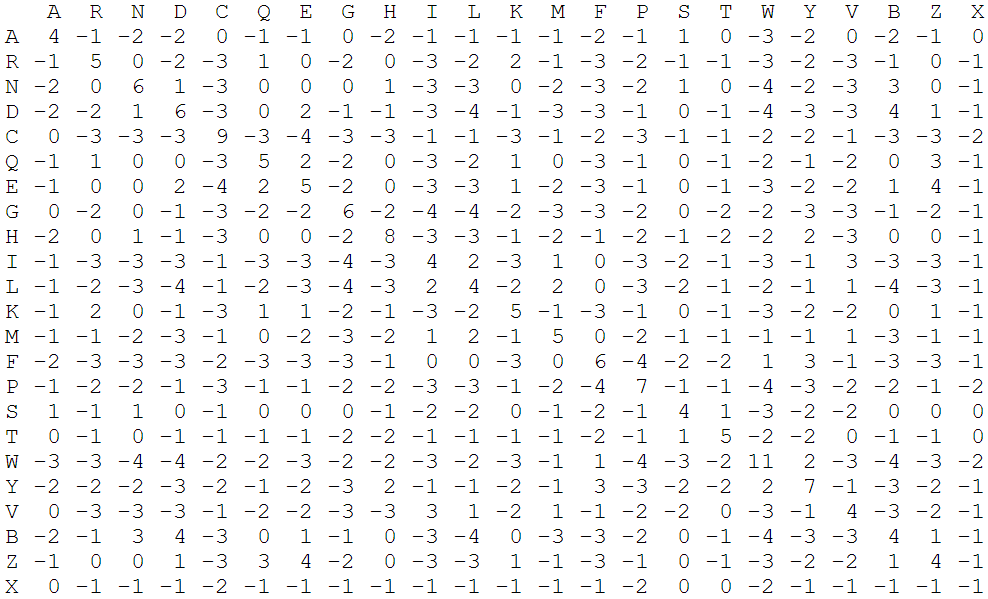
\includegraphics[width=140mm]{Figures/BLOSUM62.png}
	\caption{\fontfamily{pag}\selectfont BLOSUM62 Scoring Matrix from \url{http://www.ncbi.nlm.nih.gov/Class/FieldGuide/BLOSUM62.txt}.}
	\label{fig:blo}
\end{figure}

Sorts of sequence alignment algorithms have been studied. Next chapter will introduce two sorts of algorithms: Smith-Waterman algorithm and HMM-based algorithms. They share a very general optimization technique called dynamic programming for finding optimal alignments.

\subsection{Bioinformatics protein databases}
This part is a brief introduction of two protein sequence databases used in this thesis.

\subsubsection*{NCBI NR databse}
The NCBI (National Center for Biotechnology Information) houses a series of databases relevant to Bioinformatics. Major databases include GenBank for DNA sequences and PubMed, a bibliographic database for the biomedical literature. Other databases include the NCBI Epigenomics database. All these databases are updated daily and available online: \url{http://www.ncbi.nlm.nih.gov/guide/all/\#databases\_}.

The NR (Non-Redundant) protein database maintained by NCBI as a target for their BLAST search services is a composite of SwissProt, SwissProt updates, PIR(Protein Information Resource), PDB(Protein Data Bank). Entries with absolutely identical sequences have been merged into NR database. The PIR produces the largest, most comprehensive, annotated protein sequence database in the public domain. The PDB is a repository for the three-dimensional structural data of large biological molecules, such as proteins and nucleic acids and is maintained by Brookhaven National Laboratory, USA.

Release 2014\_04 of NCBI NR databse contains 38,442,706 sequence entries, comprising 13,679,143,700 amino acids, more than 24GB in file size \citep{NCBI}.

\subsubsection*{Swiss-Prot}
The Universal Protein Resource (UniProt) is a comprehensive resource for protein sequence and annotation data and is mainly supported by the National Institutes of Health (NIH) \citep{upr}. The UniProt databases are the UniProt Knowledgebase (UniProtKB), the UniProt Reference Clusters (UniRef), and the UniProt Archive (UniParc). 

The UniProt Knowledgebase is updated every four weeks on average and consists of two sections: 
\begin{itemize}
 \item UniProtKB/Swiss-Prot\\
 This section contains manually-annotated records with information extracted from literature and curator-evaluated computational analysis. It is also highly cross-referenced to other databases. Release 2014\_05 of 14-May-2014 of UniProtKB/Swiss-Prot contains 545,388 sequence entries, comprising 193,948,795 amino acids abstracted from 228,536 references \citep{Swiss-Prot}.
 \item UniProtKB/TrEMBL\\
 This section contains computationally analyzed records that await full manual annotation. Release 2014\_05 of 14-May-2014 of UniProtKB/TrEMBL contains 56,010,222 sequence entries, comprising 17,785,675,050 amino acids \citep{UniProtTr}.
\end{itemize}

%----------------------------------------------------------------------------------------

\section{Dynamic programming in Bioinformatics}
Dynamic Programming (DP) is an optimization technique that recursively breaks down a problem into smaller subproblems, such that the solution to the larger problem can be obtained by piecing together the solutions to the subproblems \citep{BioMach}. This section shows how the Smith-Waterman algorithms and the algorithms in HMMER use DP for sequence alignment and database searches, and then discusses the related work about acceleration on CUDA-enabled GPU.

\subsection{The Smith-Waterman algorithm}
The Smith-Waterman algorithm is designed to find the optimal local alignment between two sequences. It was proposed by Smith and Waterman \citep{SW} and enhanced by Gotoh \citep{Gotoh}. The alignment of two sequences is based on dynamic programming approach by computing the similarity score which is given in the form of similarity score matrix $H$. 

Given a query sequence $Q$ with length $L_q$ and a target sequence $T$ with length $L_t$, let $S$ be the substitution matrix and its element $S[i,j]$ be the similarity score for the combination of the $i^{th}$ residue in $Q$ and the $j^{th}$ residue in $T$. Define $G_e$ as the gap extension penalty, and $G_o$ as the gap opening penalty. These similarity scores and $G_e$, $G_o$ are pre-determined by the life sciences community. The similarity score matrix $H$ for aligning $Q$ and $T$ is calculated as 

\begin{equation*}
   E[i, j] = max 
   \begin{cases}
    E[i, j-1]-G_e\\
    H[i, j-1]-G_o
   \end{cases}
\end{equation*}
\begin{equation*}
   F[i, j] = max
   \begin{cases}
    F[i-1, j]-G_e\\
    H[i-1, j]-G_o
   \end{cases}
\end{equation*}
\begin{equation*}
   H[i, j] = max
   \begin{cases}
    0\\
    E[i, j]\\
    F[i,j]\\
    H[i-1, j-1] + S[i,j]
   \end{cases}
\end{equation*}

where $1\leqslant i \leqslant L_q$ and $1\leqslant j \leqslant L_t$. The values for $E$, $F$ and $H$ are initialized as $E[i,0] = F[0,j] = H[i,0] = H[0,j]$ when $0\leqslant i \leqslant L_q$ and $0\leqslant j \leqslant L_t$.

The maximum value of the matrix $H$ gives the similarity score between $Q$ and $T$.

%----------------------------------------------------------------------------------------
\subsection{HMMER}

\label{HMMERsect}

HMMER \citep{HMMER} is a set of applications that create a profile Hidden Markov Model (HMM) of a sequence family which can be utilized as a query against a sequence database to identify (and/or align) additional homologs of the sequence family\citep{Seq}. HMMER was developed by Sean Eddy at Washington University and has become one of the most widely used software tools for sequence homology. The main elements of this HMM-based sequence alignment package are \emph{hmmsearch} and \emph{hmmscan}. The former searches a profile HMM against a sequence database, while the latter searches a sequence against a profile HMMs database.

\subsubsection{HMM and profile HMM}

A hidden Markov model (HMM) is a computational structure for linearly analyzing sequences with a probabilistic method \citep{DicBioinfo}. HMMs have been widely used in speech signal, handwriting and gesture detection problems. In bioinformatics they have been used for applications such as sequence alignment, prediction of protein structure, analysis of chromosomal copy number changes, and gene-finding algorithm, etc \citep{BioFunc}. 

A HMM is a type of a non-deterministic finite state machine with transiting to another state and emitting a symbol under a probabilistic model.
According to \citep{SeqData}, a HMM can be defined as a 6-tuple ($A$, $Q$, $q_0$, $q_e$, $tr$, $e$) where \\[-1cm]

\begin{itemize}
\item \textbf{$A$} is a finite set (the alphabet) of symbols;
\item \textbf{$Q$} is a finite set of \emph{states};
\item \textbf{$q_0$} is the \emph{start} state and \textbf{$q_e$} is the \emph{end} state;
\item \textbf{$tr$} is the \emph{transition} mapping, which is the transition probabilities of state pairs in $Q$ $\times$ $Q$, satisfying the following two conditions: 
  \begin{enumerate}
   \item[(a)] $0 \leqslant tr(q,q') \leqslant 1$, $\forall q,q' \in Q$, and
   \item[(b)] for any given state $q$, such that:
   \begin{equation*}
    \displaystyle\sum_{q' \in Q}tr(q,q') = 1
   \end{equation*}
  \end{enumerate}
\item \textbf{$e$} is the \emph{emission} mapping, which is the emission probabilities of pairs in $Q$ $\times$ $A$, satisfying the following two conditions:
  \begin{enumerate}
   \item[(a)] $0 \leqslant e(q,x) \leqslant 1$, if it is defined, $\forall q \in Q$, and $x \in A$
   \item[(b)] for any given state $q$, if for any $x \in A$, $e(q, x)$ is defined, then $q$ is an \emph{emitting} state and
   \begin{equation*}
    \displaystyle\sum_{x \in A}e(q,x) = 1 
   \end{equation*}
   if $\forall x \in A$, $e(q, x)$ is not defined, then $q$ is a \emph{silent} state.
  \end{enumerate}
\end{itemize}

The dynamics of the system is based on Markov Chain, meaning that only the current state influences the selection of its successor – the system has no `memory' of its history. Only the succession of characters emitted is visible; the state sequence that generated the characters remains internal to the system, i.e. hidden. By this means, the name is Hidden Markov Model\citep{IntroBio}. 

Profile HMM is a variant of HMM and can be constructed from an initial multiple sequence alignment to define a set of probabilities. The symbol sequence of an HMM is an observed sequence that resembles a consensus for the multiple sequence alignment. And a protein or gen family can be defined by profile HMMs.

In Figure\ref{fig:pHMM}, the internal structure of the ``Plan 7" profile HMM used by HMMER\citep{HMMER3} shows the mechanism for generating sequences. In order to generate sequences, a profile HMM should have a set of three states per alignment column: one \emph{match} state, one \emph{insert} state and one \emph{delete} state. 
\begin{itemize}
\item \textbf{\emph{match state}} matches and emits a amino acid from the query. The probability of emitting each of the 20 amino acids is a property of the model. 
\item \textbf{\emph{insert state}} allows the insert of one or more amino acids. The emission probability of this state is computed either from a background distribution of amino acids or from the observed insertions in the alignment.
\item \textbf{\emph{delete state}} skips the alignment column and emits a blank. Entering this state corresponds to gap opening, and the probabilities of these transitions reflect a position-specific gap penalty.
\end{itemize}

\begin{figure}[!htb]
	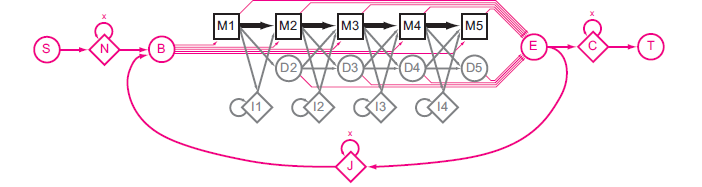
\includegraphics[width=150mm]{Figures/pHMM.png}
	\caption{\fontfamily{pag}\selectfont Profile HMM architecture used by HMMER\citep{HMMER3}.}
	\label{fig:pHMM}
\end{figure}

The structure begins at Start(S), and follows some chain of arrows until arriving at Termination(T). Each arrow transits to a state of the system. 
At each state, an action can be taken either as (1) emitting a residue, or (2) selecting an arrow to the next state. The action and the selection of successor state are governed by sets of probabilities\citep{IntroBio}.
The linear core model has five sets of match (M), insert (I) and delete (D) states. Each M state represents one consensus position and a set of M, I, D states is the main element of the model and is referred to as a ``node''� in HMMER. Additional flanking states (marked as N, C, and J) emit zero or more residues from the background distribution, modelling nonhomologous regions preceding, following, or joining homologous regions aligned to the core model. Start (S), begin (B), end (E) and termination (T) states are non-emitting states.

A profile HMM for a protein family can be used to compare with target sequences, and classify sequences that are members of the family and those which are not\citep{ProteinBio}. 
A common application of profile HMMs is used to search a profile HMM against a sequence database. Another application is the query of a single protein sequence of interest against a database of profile HMMs.

\subsubsection{Viterbi algorithm in HMMER2}

\label{ViterbiSub}

In HMMER2, both \emph{hmmsearch} and \emph{hmmpfam} rely on the same core Viterbi algorithm for their scoring function which is named as \emph{P7Viterbi} in codes.

To find whether a sequence is member of the family described by a HMM, we compare the sequence with the HMM. We use an algorithm known as Viterbi to find one path that has the maximum probability of the HMM generating the sequence. Viterbi is a dynamic programming algorithm. Let $V_{i,j}$ be the maximum probability of a path from the start state $S_i$ ending at state $S_j$ and generating the prefix $q_{1...j}$ of the target sequence. $V_{i+1,j}$ is found by the recurrence:

\begin{equation*}
   \displaystyle V_{i+1,j} = \max_{0 \leqslant k \leqslant j-1} \big ( V_{i,k} P(k,j)P(q_{i+1} |j) \big )
\end{equation*}

% max |x| = 
%     \begin{cases}
%     \quad -x & \text{if } x < 0,\\
%     0 & \text{if } x = 0,\\
%     x & \text{if } x > 0.
%     \end{cases}
%     max = \left\{
% \begin{array}{rl}
% -x & \text{if } x < 0,\\
% 0 & \text{if } x = 0,\\
% x & \text{if } x > 0.
% \end{array} \right.

Define $a[i,j]$ as the transition probability from state $i$ to $j$ and $e_i$ as emission probability in state $i$.
Define $V_j^M(i)$ as the log-odds score of the optimal path matching subsequence $x_{1...i}$ to the submodel up to state $j$, ending with $x_i$ being emitted by \emph{match} state $M_j$. Similarly $V_j^I(i)$ is the score of the optimal path ending in $x_i$ being emitted by \emph{insert} state $I_j$, and $V_j^D(i)$ for the optimal path ending in \emph{delete} state $D_j$. $q_{x_i}$ is the probability of $x_i$. Then we can write the Viterbi general equation\citep{BioSeq}:

\begin{equation*}
   V_j^M(i) = \log\frac{e_{M_j}(x_i)}{q_{x_i}} + max 
   \begin{cases}
   V_{j-1}^M(i-1) + \log a[M_{j-1},M_j]\\
   V_{j-1}^I(i-1) + \log a[I_{j-1},M_j]\\
   V_{j-1}^D(i-1) + \log a[D_{j-1},M_j]
   \end{cases}
\end{equation*}

\begin{equation*}
   V_j^I(i) = \log\frac{e_{I_j}(x_i)}{q_{x_i}} + max 
   \begin{cases}
   V_j^M(i-1) + \log a[M_j,I_j]\\
   V_j^I(i-1) + \log a[I_j,I_j]
   \end{cases} 
\end{equation*}

\begin{equation*}
   V_j^D(i) = max 
   \begin{cases}
   V_{j-1}^M(i) + \log a[M_{j-1},D_j]\\
   V_{j-1}^D(i) + \log a[D_{j-1},D_j]
   \end{cases}  
\end{equation*}

Based on the above equations, we can write the efficient pseudo code of Viterbi algorithm, as shown in Algorithm\ref{Viterbi} \citep{FPGA}.  The inner loop of the code contains three two dimensional matrices (M, I, D), which calculate scores of all node positions involved in the main models for each of the residue. The outer loop consists of flanking and special states calculated in the one dimensional arrays N, B, C, J, E.

\renewcommand{\thepseudonum}{\roman{pseudonum}}
\begin{pseudocode}{Viterbi}{ }
\label{Viterbi}
\COMMENT{Initialization}\\
N[0] \GETS 0; \ \  B[0] \GETS tr(N, B)\\
E[0] \GETS C[0] \GETS J[0] \GETS -\infty\\
\COMMENT{for every sequence residue i}\\
\FOR i \GETS 1 \TO L_t \DO
\BEGIN
  N[i] \GETS N[i-1] + tr(N, N)\\
  B[i] \GETS max 
  \begin{cases}
   N[i-1] + tr(N, B)\\
   J[i-1] + tr(J, B)
  \end{cases}\\
  M[i,0] \GETS I[i,0] \GETS D[i,0] \GETS -\infty\\
  \COMMENT{For every model position j from 1 to $L_q$}\\
  \FOR j \GETS 1 \TO L_q \DO
  \BEGIN
    M[0, j] \GETS I[0, j] \GETS D[0, j] \GETS -\infty\\
    M[i, j] \GETS e(M_j, S[i]) + max 
    \begin{cases}
     M[i-1, j-1] + tr(M_{j-1}, M_j)\\
     I[i-1, j-1] + tr(I_{j-1}, M_j)\\
     D[i-1, j-1] + tr(D_{j-1}, M_j)\\
     B[i-1] + tr(B, M_j)
    \end{cases}\\
    I[i, j] \GETS e(I_j, S[i]) + max
    \begin{cases}
     M[i-1, j] + tr(M_j, I_j)\\
     I[i-1, j] + tr(I_j, I_j)
    \end{cases}\\
    D[i, j] \GETS max
    \begin{cases}
     M[i, j-1] + tr(M_{j-1}, D_j)\\
     D[i, j-1] + tr(D_{j-1}, D_j)
    \end{cases}\\
  \END\\
  E[i] \GETS max\{M[i,j] + tr(M_j, E)\} \ \  (j \GETS 0 \TO L_q)\\
  J[i] \GETS max 
  \begin{cases}
   J[i-1] + tr(J, J)\\
   E[i-1] + tr(E, J)
  \end{cases}\\
  C[i] \GETS max
  \begin{cases}
   C[i-1] + tr(C, C)\\
   E[i-1] + tr(E, C)
  \end{cases}\\
\END\\
\COMMENT{Termination: }\\
\RETURN {T(S,M) \GETS C[L_t] + tr(C,T)}
\end{pseudocode}

From Algorithm\ref{Viterbi}, we can see the fundamental task of the Viterbi algorithm for Biological Sequence Alignment is to calculate three DP(Dynamic Programming) matrices: $M[{ }]$ for Match state, $I[{ }]$ for Insert state and $D[{ }]$ for Delete state. Each DP matrix consisting of $(L_t+1) * (L_q+1)$ blocks, where each value of block is dependent on the value of previous block. As shown in Figure\ref{fig:dpV}, the Match state $M[i,j]$ depends on the upper-left block $M[i-1, j-1]$, $I[i-1, j-1]$ and $D[i-1, j-1]$; the Insert state $I[i,j]$ depends on the left block $M[i-1, j]$ and $I[i-1, j]$; and the Delete state depends on the upper block $M[i, j-1]$ and $D[i, j-1]$.

\begin{figure}[!htb]
\centering
	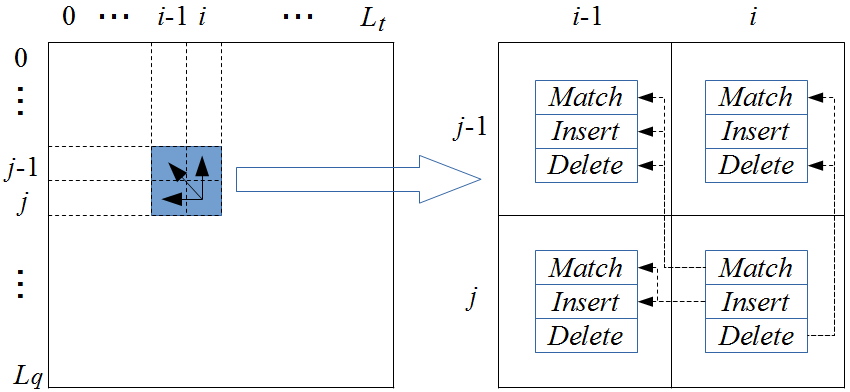
\includegraphics[width=120mm]{Figures/dpViterbi.png}
	\caption{\fontfamily{pag}\selectfont \textbf{The DP matrix calculated in Viterbi algorithm.} 
The rectangle on the left represents the whole matrix to be calculated by the Viterbi algorithm, and the right rectangle of the figure shows the process of updating a single block of the matrix.}
	\label{fig:dpV}
\end{figure}

\subsubsection{MSV algorithm in HMMER3}

\label{MSVsub}

HMMER3 is near rewrite of the earlier HMMER2 package, with the aim of improving the speed of profile HMM searches. The main performance gain is due to a heuristic algorithm called MSV filter, for Multiple (local, ungapped) Segment Viterbi. MSV is implemented in SIMD(Single-Instruction Multiple-Data) vector parallelization instructions and is about 100-fold faster than HMMER2.

\begin{figure}[!htb]
	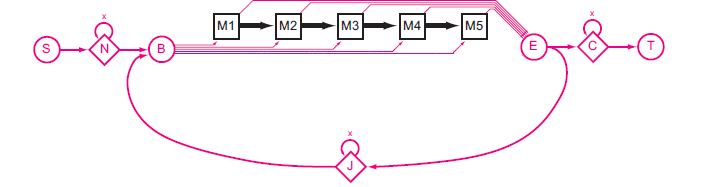
\includegraphics[width=150mm]{Figures/pHMM_msv.png}
	\caption{\fontfamily{pag}\selectfont MSV profile: multiple ungapped local alignment segments \citep{HMMER3}.}
	\label{fig:pMSV}
\end{figure}

Figure\ref{fig:pMSV} illustrates the MSV profile architecture. Compared with Figure\ref{fig:pHMM}, the MSV corresponds to the virtual removal of the delete and insert states. All match-match transition probabilities are treated as 1.0. The rest parameters remains unchanged. So this model generates sequences containing one or more ungapped local alignment segments. The pseudo code of MSV score algorithm is simplified and shown in Algorithm\ref{MSV}.

Figure\ref{fig:dpMSV} illustrates an example of an alignment of a MSV profile HMM model (length $L_q = 14$) to a target sequence (length $L_t=22$). A path to generate the target sequence with the profile HMM model is shown through a dynamic programming (DP) matrix. The model identifies two high-scoring ungapped alignment segments, as shown in black dots, indicating residues aligned to profile match states. All other residues are assigned to N, J, and C states in the model, as shown in orange dots. Unfilled dot indicates a ``mute'' non-emitting state or state transition.

\begin{figure}[!htb]
\centering
	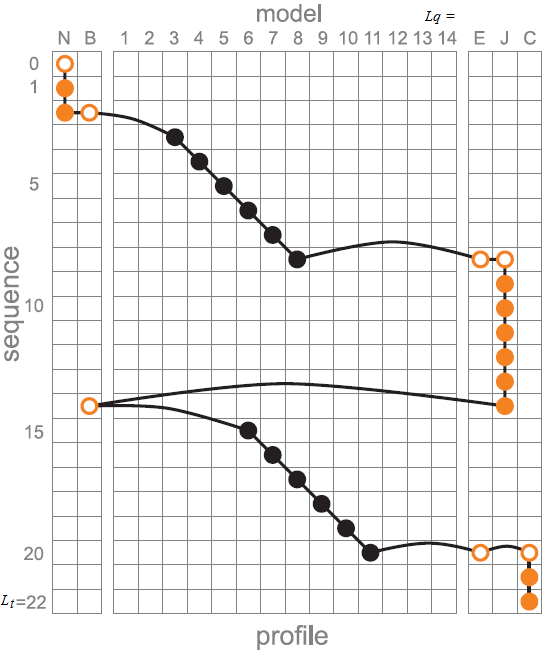
\includegraphics[width=100mm]{Figures/dpMSV.png}
	\caption{\fontfamily{pag}\selectfont \textbf{Example of an MSV path in DP matrix \citep{HMMER3}.} 
An alignment of a MSV profile HMM model (length $L_q = 14$) to a target sequence (length $L_t=22$). A path from top to bottom is through a dynamic programming (DP) matrix. The model identifies two high-scoring ungapped alignment segments, as shown in black dots, indicating residues aligned to profile match states. All other residues are assigned to N, J, and C states in the model, as shown in orange dots. Unfilled dot indicates a ``mute'' non-emitting state or state transition.}
	\label{fig:dpMSV}
\end{figure}

\begin{pseudocode}{MSV}{ }
\label{MSV}
\COMMENT{Initialization}\\
N[0] \GETS 0; \ \  B[0] \GETS tr(N, B)\\
E[0] \GETS C[0] \GETS J[0] \GETS -\infty\\
\COMMENT{for every sequence residue i}\\
\FOR i \GETS 1 \TO L_t \DO
\BEGIN
  N[i] \GETS N[i-1] + tr(N, N)\\
  B[i] \GETS max 
  \begin{cases}
   N[i-1] + tr(N, B)\\
   J[i-1] + tr(J, B)
  \end{cases}\\
  M[i,0] \GETS -\infty\\
  \COMMENT{For every model position j from 1 to $L_q$}\\
  \FOR j \GETS 1 \TO L_q \DO
  \BEGIN
    M[0, j] \GETS -\infty\\
    M[i, j] \GETS e(M_j, S[i]) + max 
    \begin{cases}
     M[i-1, j-1]\\
     B[i-1] + tr(B, M_j)
    \end{cases}\\
  \END\\
  E[i] \GETS max\{M[i,j] + tr(M_j, E)\} \ \  (j \GETS 0 \TO L_q)\\
  J[i] \GETS max 
  \begin{cases}
   J[i-1] + tr(J, J)\\
   E[i-1] + tr(E, J)
  \end{cases}\\
  C[i] \GETS max
  \begin{cases}
   C[i-1] + tr(C, C)\\
   E[i-1] + tr(E, C)
  \end{cases}\\
\END\\
\COMMENT{Termination: }\\
\RETURN {T(S,M) \GETS C[L_t] + tr(C,T)}
\end{pseudocode}

\subsubsection{SIMD vectorized MSV in HMMER3}
\label{SSE2}

Single-Instruction Multiple-Data (SIMD) instruction is able to perform the same operation on multiple pieces of data in parallel. The first widely-deployed desktop SIMD was with Intel's MMX extensions to the x86 architecture in 1996. In 1999, Intel introduced Streaming SIMD Extensions (SSE) in Pentium III series processors. The modern SIMD vector instruction sets use 128-bit vector registers to compute up to 16 simultaneous operations. Due to the huge number of iterations in the Smith-Waterman algorithm calculation, using SIMD instructions to reduce the number of instructions needed to perform one cell calculation has a significant impact on the execution time. Several SIMD vector parallelization methods have been described for accelerating SW dynamic programming. 

In 2000, Rognes and Seeberg presented an implementation of the SW algorithm running on the Intel Pentium processor using the MMX SIMD instructions \citep{SW-SIMD}. They used a query profile parallel to the query sequence for each possible residue. A query profile was pre-calculated in a sequential layout just once before searching database. A six-fold speedup was reported over an optimized non-SIMD implementation. 

In 2007, Farrar presented an efficient vector-parallel approach called striped layout for vectorizing SW algorithm \citep{SW-SSE2}. He designed a striped query profile for SIMD vector computation. He used Intel SSE2 to implement his design. A speedup of 2-8 times was reported over the Rognes and Seeberg SIMD non-stripped implementations.

Inspired by Farrar, in HMMER3\citep{HMMER3}, Sean R. Eddy used a remarkably efficient stripped vector-parallel approach to calculate MSV alignment scores. To maximize parallelism, he implemented MSV as a 16-fold parallel calculation with score values stored as 8-bit byte integers. He used SSE2 instructions on Intel-compatible systems and Altivec/VMX instructions on PowerPC systems.

Figure\ref{fig:strip} shows the stripped pattern. The query profile HMM of length $L_q$ is divided into vectors with equal length $L_v$. The vector length $L_v$ is equal to the number of elements being processed in the 128-bit SIMD register. MSV processes 8-bit byte integer with $L_v$ = 128/8 = 16. In a row-vectorized implementation, the query profile HMM is stored in the vectorized dynamic programming matrix dp. The dp stores $L_q$ cells in $L_Q$ vectors which is numbered as $q = 1...L_Q$, where $L_Q = (L_q+L_v-1)/L_v$. Figure\ref{fig:strip} illustrates $L_q$ cells assigned to $L_Q$ vectors in a non-sequential way. For simple illustration, $L_v = 4, L_q = 14$, and $L_Q = 4$.

\begin{figure}[!htb]
	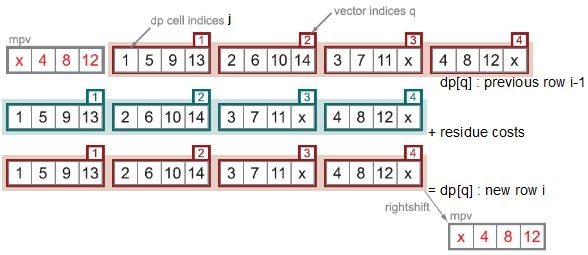
\includegraphics{Figures/msv_vector.jpg}
	\caption{\fontfamily{pag}\selectfont Illustration of striped indexing for SIMD vector calculations\citep{HMMER3}.}
	\label{fig:strip}
\end{figure}

In Smith-Waterman and Viterbi dynamic programming, the calculation of each cell $(i, j)$ in the dp is dependent on previously calculated cells $(i-1, j), (i, j-1)$ and $(i-1, j-1)$. However, in MSV algorithm, the \emph{delete} and \emph{insert} states have been removed and only ungapped diagonals need calculating, so the calculation of each cell $(i, j)$ requires only previous $(i-1, j-1)$. In Figure\ref{fig:strip}, the top red row shows the previous row $i-1$ for the cells $j-1$, which is needed for calculating each new cell $j$ in a new row $i$. 

Striping method can remove the SIMD register data dependencies. As can be seen in the Figure\ref{fig:strip}, with striped indexing, vector $q-1$ contains exactly the four $j-1$ cells needed to calculate the four cells $j$ in a new vector $q$ on a new blue row of the dp matrix. For example, when we calculate cells $j=(2,6,10,14)$ in vector $q=2$, we access the previous row’s vector $q-1=1$ which contains the cells we need in the order we need them, $j-1=(1,5,9,13)$ (the vector above). 

\begin{figure}[!htb]
\centering
	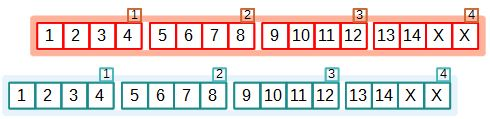
\includegraphics[width=110mm]{Figures/msv_nostrip.jpg}
	\caption{\fontfamily{pag}\selectfont Illustration of linear indexing for SIMD vector calculations.}
	\label{fig:nostrip}
\end{figure}

Instead, if we indexed cells into vectors in the linear order ($j=1,2,3,4$ in vector $q=1$ and so on), as shown in Figure\ref{fig:nostrip}, there is no such correspondence of $(q,q-1)$ with four $(j-1,j)$, and each calculation of a new vector $q$ would require extra expensive operations, such as shifting or rearranging cell values inside the previous row's vectors. By using the striped query access, only one shift operation is needed per row as shown in \ref{fig:strip}. Outside the inner loop(for $q = 1$ to $L_Q$), the last vector on each finished row is right-shifted (mpv, in grey with red cell $j$ indices) and used to initialize the next row calculation.

The pseudo code for the implementation is shown in Algorithm\ref{MSV-SIMD}

\begin{pseudocode}{MSV-SIMD}{ }
\label{MSV-SIMD}
\COMMENT{Initialization}\\
xJ \GETS 0; \ \  dp[q] \GETS vec\_splat(0) \  (q \GETS 0 \TO L_Q-1)\\
xB \GETS base + tr(N, B)\\
xBv \GETS vec\_adds(xB, tr(B, M))\\
\COMMENT{for every sequence residue i}\\
\FOR i \GETS 1 \TO L_t \DO
\BEGIN
  xEv \GETS vec\_splat(0)\\
  mpv \GETS vec\_rightshift(dp[L_Q-1])\\
  \FOR q \GETS 0 \TO L_Q-1 \DO
  \BEGIN
    \COMMENT{temporary  storage of 1 current row value in progress}\\
    tmpv \GETS vec\_max(mpv, xBv)\\
    tmpv \GETS vec\_adds(tmpv, e(M_j, S[i]))\\
    xEv \GETS vec\_max(xEv, tmpv)\\
    mpv \GETS dp[q]\\
    dp[q] \GETS tmpv\\
  \END\\
  xE \GETS vec\_hmax(xEv)\\
  xJ \GETS max 
  \begin{cases}
   xJ\\
   xE + tr(E, J)
  \end{cases}\\
  xB \GETS max 
  \begin{cases}
   base\\
   xJ + tr(J, B)
  \end{cases}\\
\END\\
\COMMENT{Termination: }\\
\RETURN {T(S,M) \GETS xJ + tr(C,T)}
\end{pseudocode}

Five pseudocode vector instructions for operations on 8-bit integers are used in the pseudo code. Either scalars $x$ or vectors v containing 16 8-bit integer elements numbered $v[0]...v[15]$. Each of these operations are either available or easily constructed in Intel SSE2 intrinsics as shown in the following table.

% \begin{minipage}{\textwidth}
% \begin{center}
% \begin{tabular}{|c|c|c|}\hline
% \shortstack{\textbf{Pseudocode} \\ SSE2 code in C} & \textbf{Operation} & \textbf{Definition}\\\hline
% \shortstack{\textbf{v = vec\_splat(x)} \\ v = \_mm\_set1\_epi8(x)} & assignment & $v[z] = x$\\\hline
% \shortstack{\textbf{v = vec\_adds(v1, v2)} \\ v = \_mm\_adds\_epu8(v1, v2)} & saturated addition & $v[z] = min$
% $\begin{cases}
%   2^8-1\\
%   v1[z]+v2[z]
% \end{cases}$\\\hline
% \shortstack{\textbf{v1 = vec\_rightshift(v2)} \\ v1 = \_mm\_slli\_si128(v2, 1)} & right shift & \shortstack{$v1[z] = v2[z-1](z=16...1)$; \\ $v1[0]=0;$}\\\hline
% \shortstack{\textbf{v = vec\_max(v1, v2)} \\ v = \_mm\_max\_epu8(v1, v2)} & max & $v[z] = max(v1[z], v2[z])$\\\hline
% \shortstack{\textbf{x = vec\_hmax(v)} \\ -} & horizontal max & $x = max_zv[z]$\\\hline
% \end{tabular}
% \end{center}
% \end{minipage}


\begin{table}[H]
\centering
\begin{tabular}{|c|c|c|}\hline
\shortstack{\textbf{Pseudocode} \\ SSE2 intrinsic in C} & \textbf{Operation} & \textbf{Definition}\\\hline
\shortstack{\textbf{v = vec\_splat(x)} \\ v = \_mm\_set1\_epi8(x)} & assignment & $v[z] = x$\\\hline
\shortstack{\textbf{v = vec\_adds(v1, v2)} \\ v = \_mm\_adds\_epu8(v1, v2)} & saturated addition & $v[z] = min$
$\begin{cases}
  2^8-1\\
  v1[z]+v2[z]
\end{cases}$\\\hline
\shortstack{\textbf{v1 = vec\_rightshift(v2)} \\ v1 = \_mm\_slli\_si128(v2, 1)} & right shift & \shortstack{$v1[z] = v2[z-1](z=15...1)$; \\ $v1[0]=0;$}\\\hline
\shortstack{\textbf{v = vec\_max(v1, v2)} \\ v = \_mm\_max\_epu8(v1, v2)} & max & $v[z] = max(v1[z], v2[z])$\\\hline
\shortstack{\textbf{x = vec\_hmax(v)} \\ -} & horizontal max & $x = max(v[z]),z=0...15$\\\hline
\end{tabular}
\caption{\fontfamily{pag}\selectfont\textbf{SSE2 intrinsics for pseudocode in Algorithm\ref{MSV-SIMD}} The first column is pseudocode and its corresponding SSE2 intrinsic in C language. Because x86 and x86-64 use little endian, \textbf{vec\_rightshift()} means using a left bit shift intrinsic \textbf{\_mm\_slli\_si128()} to do right shift. No SSE2 intrinsic is corresponding to \textbf{vec\_hmax()}. Shuffle intrinsic \textbf{\_mm\_shuffle\_epi32} and \textbf{\_mm\_max\_epu8} can be combined to implement \textbf{vec\_hmax()}.\label{tab.SSE2}}
\end{table}


%----------------------------------------------------------------------------------------

\section{CUDA accelerated sequence alignment}
\label{CUDASeqAlign}

In November 2006, NVIDIA\textregistered introduced CUDA\texttrademark (Compute Unified Device Architecture), a general purpose parallel computing platform and programming model that enables users to write scalable multi-threaded programs in NVIDIA GPUs. Nowadays there exist alternatives to CUDA, such as OpenCL \citep{OpenCL}, Microsoft Compute Shader\citep{Shader}. These are mostly similar, but as CUDA is the most widely used and more mature, this thesis will focus on that.

This section firstly overviews CUDA programming model, then reviews recent studies on accelerating Smith-waterman algorithm and HMM-based algorithms on CUDA-enabled GPU.

\subsection{Overview of CUDA programming model}
\subsubsection{Streaming Multiprocessors}
A GPU consists of one or more SMs(Streaming Multiprocessors). Quadro K4000 used in our research has 4 SMs. Each SM contains the following specific features \citep{CUDAHand}:

\begin{itemize}
 \item Execution units to perform integer and single- or double-precision floating-point arithmetic, Special function units (SFUs) to compute single-precision floating-point transcendental functions
 \item Thousands of registers to be partitioned among threads
 \item Shared memory for fast data interchange between threads
 \item Several caches, including constant cache, texture cache and L1 cache
 \item A warp scheduler to coordinate instruction dispatch to the execution units
\end{itemize}

The SM has been evolving rapidly since the introduction of the first CUDA-enabled GPU device in 2006, with three major Compute Capability 1.x, 2.x, and 3.x, corresponding to Tesla-class, Fermi-class, and Kepler-class hardware respectively. Table\ref{tab.sm} summarizes the features introduced in each generation of the SM hardware \citep{CUDAHand}.

\begin{table}[H]
\begin{tabular}[t]{|c|c|}\hline
\shortstack{\textbf{Compute}\\ \textbf{Capability} } & \textbf{Features introduced} \\\hline
SM 1.x & \shortstack[l]{Global memory atomics; mapped pinned memory; debuggable;\\ atomic operations on shared memory; Double precision} \\\hline
{SM 2.x} & \shortstack[l]{64-bit addressing; L1 and L2 cache; concurrent kernel execution;\\ global atomic add for single-precision floating-point values;\\ Function calls and indirect calls in kernels} \\\hline
SM 3.x & \shortstack[l]{SIMD Video Instructions; Increase maximum grid size; warp shuffle;\\ Bindless textures (``texture objects''); read global memory via texture;\\ faster global atomics; 64-bit atomic min, max, AND, OR, and XOR;\\ dynamic parallelism} \\\hline
\end{tabular}
\caption{\fontfamily{pag}\selectfont Features per Compute Capability\label{tab.sm}}
\end{table}

\subsubsection{CUDA thread hierarchy}
The execution of a typical CUDA program is illustrated in Figure\ref{fig:exeCUDA} The CPU host invokes a GPU kernel in-line with the triple angle-bracket $<<<$  $>>>$ syntax from CUDA C/C++ extension code. The kernel is executed N times in parallel by N different CUDA threads. All the threads that are generated by a kernel during an invocation are collectively called a \emph{grid}. Figure\ref{fig:exeCUDA} shows the execution of two grids of threads.

\begin{figure}[!htb]
	\centering
	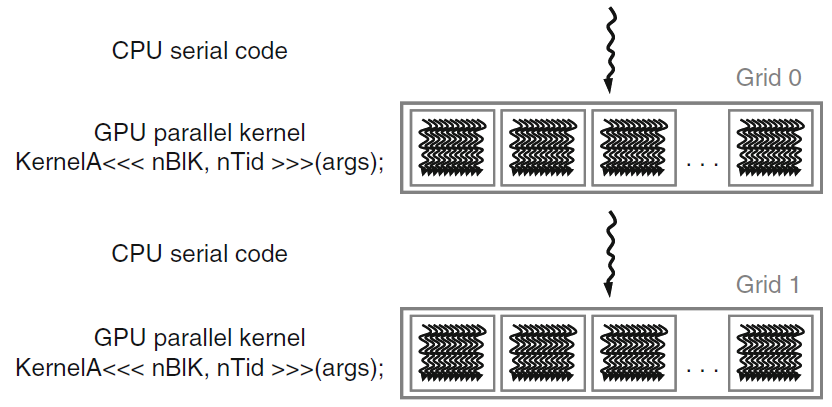
\includegraphics[totalheight=0.2\textheight]{Figures/exeCUDA.png}
	\caption{\fontfamily{pag}\selectfont Execution of a CUDA program\citep{Kirk}.}
	\label{fig:exeCUDA}
\end{figure}

Threads in a grid are organized into a two-level hierarchy, as illustrated in Figure\ref{fig:grid}. At the top level, each grid consists of one or more thread blocks. All blocks in a grid have the same number of threads and are organized into a one, two, or three-dimensional \emph{grid} of thread blocks.

\begin{figure}[!htb]
	\centering
	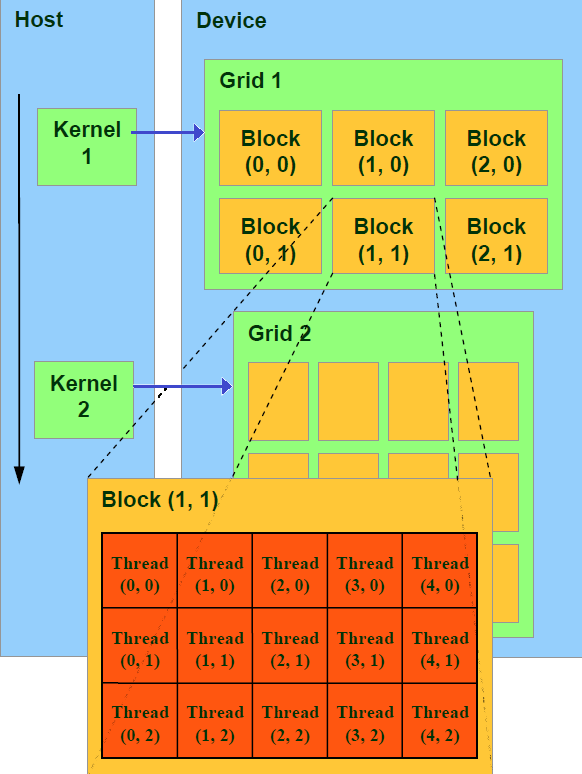
\includegraphics[totalheight=0.4\textheight]{Figures/gridBlock.png}
	\caption{\fontfamily{pag}\selectfont CUDA thread organization\citep{Zeller}.}
	\label{fig:grid}
\end{figure}

Each block can be identified by an index accessible within the kernel through the built-in \emph{blockIdx} variable. The dimension of the thread block is accessible within the kernel through the built-in \emph{blockDim} variable.

The threads in a block are executed by the same multiprocessor within a GPU. They can cooperate by sharing data through some shared memory and by synchronizing their execution to coordinate memory accesses. Each block can be scheduled on any of the available multiprocessors, in any order, concurrently or sequentially, so that a compiled CUDA program can execute on any number of multiprocessors. On the hardware level, a block's threads are executed in parallel as \emph{warps} which name originate from \emph{weaving loom}. A warp consists of 32 threads.

\subsubsection{CUDA memory hierarchy}
\label{cudaMemH}
Besides the threading model, another thing that makes CUDA programming different from a general purpose CPU is its memory spaces, including registers, local, shared, global, constant and texture, as shown in Figure\ref{fig:cudaMem}

\begin{figure}[!htb]
	\centering
	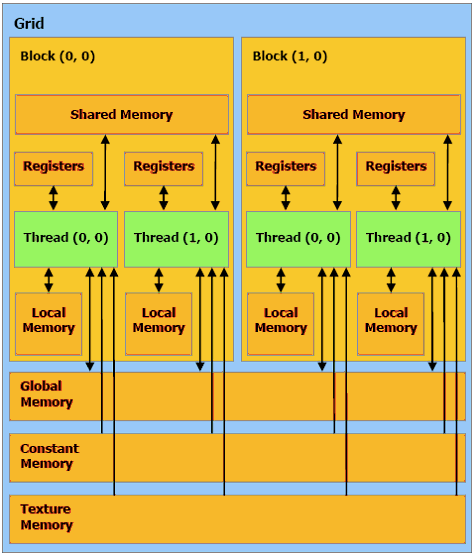
\includegraphics[totalheight=0.4\textheight]{Figures/cudaMem.png}
	\caption{\fontfamily{pag}\selectfont CUDA memory organization\citep{Zeller}.}
	\label{fig:cudaMem}
\end{figure}

CUDA memory spaces have different characteristics that reflect their distinct usages in CUDA applications as summarized in Table\ref{tab.mem} \citep{CUDABest}.

\begin{table}[H]
\centering
\begin{tabular}{|c|c|c|c|c|c|c|}\hline
\textbf{Memory} & \textbf{Location} & \textbf{Cached} & \textbf{Access} & \textbf{Scope} & \textbf{Speed} & \textbf{Lifetime} \\\hline
Register & On chip & n/a & R/W & 1 Thread & 1 & Thread \\\hline
Local & Off chip & \dag & R/W & 1 Thread & $\sim 2 - 16$ & Thread \\\hline
Shared & On chip & n/a & R/W & \shortstack{All threads\\ in block} & $\sim 2 - 16$ & Block \\\hline
Global & Off chip & \dag & R/W & \shortstack{All threads\\ + host} & 200+ & Host allocation \\\hline
Constant & Off chip & Yes & R & \shortstack{All threads\\ + host} & $2 - 200$ & Host allocation \\\hline
Texture & Off chip & Yes & R & \shortstack{All threads\\ + host} & $2 - 200$ & Host allocation \\\hline
\end{tabular}
\caption{\fontfamily{pag}\selectfont \textbf{Salient Features of GPU Device Memory.} \textbf{Speed} column is the relative speed in number of instructions. {\dag} means it is cached only on devices of above compute capability 2.x. \label{tab.mem}}
\end{table}

\subsubsection{CUDA tools}
\label{cudaTools}

The NVIDIA CUDA Toolkit provides a comprehensive development environment for C/C++ developers building GPU-accelerated applications. The CUDA Toolkit is available at \url{https://developer.nvidia.com/cuda-toolkit}, including a compiler \emph{nvcc} for NVIDIA GPUs, math libraries, and tools for debugging and optimizing the performance of CUDA applications.

\textbf{Nsight Eclipse Edition}\\
NVIDIA Nsight Eclipse Edition is a full-featured IDE powered by the Eclipse platform that provides an all-in-one integrated programming environment for editing, building, debugging and profiling CUDA C/C++ applications. Nsight Eclipse Edition supports a rich set of commercial and free plugins.
Nsight Eclipse Edition ships as part of the CUDA Toolkit Installer for Linux and Mac at \url{https://developer.nvidia.com/nsight-eclipse-edition}.

\textbf{NVIDIA Nsight Visual Studio Edition}\\
NVIDIA provides Nsight Visual Studio Edition to integrate seamlessly into Microsoft Visual Studio environment at\\ \url{https://developer.nvidia.com/nvidia-nsight-visual-studio-edition}. It can\\ build, debug, profile and trace heterogeneous compute and graphics applications using CUDA C/C++, OpenCL, DirectCompute, Direct3D, and OpenGL.

\textbf{Profiling tools}\\
 NVIDIA® provides profiling tools to help execute the kernels in question under the watchful gaze, which are publicly available as a separate download on the CUDA Zone website \citep{CUDAzone}.
 
% \begin{table}[H]
% \centering
% \begin{tabular}{|c|c|c|c|}\hline
% \shortstack{\textbf{Tools Name}} & \shortstack{\textbf{Command}} & \shortstack{\textbf{OS}} & \shortstack{\textbf{User interface}}\\\hline
% nvprof & nvprof & \shortstack{Linux, Mac OS X\\ and Windows} & command-line\\\hline
% Visual Profiler & nvvp & \shortstack{Linux, Mac OS X\\ and Windows} & graphical \\\hline
% Nsight™ Ecipse Edition & nsight & Linux and Mac OSX & graphical\\\hline
% \shortstack{NVIDIA® Nsight™ \\ Visual Studio Edition} & -\tablefootnote[12]{Integrated into Microsoft Visual Studio} & Windows & graphical\\\hline
% Parallel Nsight™ & - & Windows & graphical\\\hline
% \end{tabular}
% \caption{CUDA profiling tools\label{tab.prof}}
% \end{table}

\begin{table}[H]
\centering
\begin{tabular}{|c|c|c|c|}\hline
\shortstack{\textbf{Tools Name}} & \shortstack{\textbf{OS}} & \shortstack{\textbf{User interface}}\\\hline
nvprof & \shortstack{Linux, Mac OS X\\ and Windows} & command-line\\\hline
Visual Profiler & \shortstack{Linux, Mac OS X\\ and Windows} & graphical \\\hline
Nsight™ Ecipse Edition & Linux and Mac OSX & graphical\\\hline
\shortstack{NVIDIA® Nsight™ \\ Visual Studio Edition} & Windows & graphical\\\hline
Parallel Nsight™ & Windows & graphical\\\hline
\end{tabular}
\caption{\fontfamily{pag}\selectfont {CUDA profiling tools}\label{tab.prof}}
\end{table}

\textbf{Nvidia-SMI}\\
The NVIDIA System Management Interface (nvidia-smi) is a command line utility that helps managing and monitoring GPU devices. It ships with NVIDIA GPU display drivers on Linux and Windows. This utility allows administrators to query GPU device state and modify GPU device state. It can also report control aspects of GPU execution, such as whether ECC is enabled and how many CUDA contexts can be created on a given GPU.

% http://docs.nvidia.com/cuda/profiler-users-guide/#axzz32CP5hrTb
%----------------------------------------------------------------------------------------

\subsection{CUDA accelerated Smith-Waterman}
The Smith-Waterman algorithm for sequence alignment uses dynamic programming method for sequence alignment, which is also the characteristic of HMM-based algorithms. In this section, we review the techniques used in parallelizing Smith-Waterman on a CUDA-enabled GPU and these techniques will be evaluated for accelerating MSV algorithm in Chapter \ref{CUDAHMMER3}.

\subsubsection*{Parallelism strategy applied}
As explained in Section\ref{impl}, parallel computing has two types of parallelism: task-based and data-based parallelism. SW algorithm is used for finding similarity among protein sequence database with dynamic programming method. The application is particularly well-suited for many-core architectures due to the parallel nature of sequence database searches. Among 8 articles reviewed here, 7 articles, i.e. \citep{Manavski}, \citep{SW++}, \citep{Akoglu}, \citep{Ligowski}, \citep{SW++2}, \citep{Kentie} and \citep{SW++3} used task-based parallelism to process each target sequence independently with a single GPU thread. Task-based parallelism removes the need for inter-thread communications or, even worse, inter-multiprocessor communications. This also simplifies implementation and testing. This approach was taken by most of studies and more efforts were put on optimizing CUDA kernel execution.

For data-based parallelism, \citep{Saeed} formulated parallel version of the Smith-Waterman algorithm so that the calculations
can be performed in parallel one row (or column) of similarity matrix at a time. They exploited approach of parallelizing multiple GPUs with using MPI (Message Passing Interface) parallel technique over 100 Mb Ethernet to extend work to multiple GPUs.

\citep{SW++} investigated the two parallelism approaches for parallelizing the sequence database searches using CUDA. They found task-based parallelism can achieve better performance although it needs more device memory than data-based. They used data-based parallelism to support longest query/target sequences. Each task was assigned to one thread block and all threads in the thread block cooperate to perform the task in parallel, exploiting the parallel characteristics of cells in the minor diagonals of similarity matrix. 

\subsubsection*{Processing target sequences database}
In order to achieve high efficiency for task-based parallelism, the run time of all threads in a thread block should be roughly identical. Therefore many studies often sorted sequences databases by length of sequences. Thus, for two adjacent threads in a thread warp, the difference value between the lengths of the associated sequences is minimized, thereby balancing a similar workload over threads in a warp.
\citep{Manavski}, \citep{Akoglu}, \citep{SW++3} presorted database in ascending order.

\citep{Ligowski} presorted database in descending order and organized in blocks consisting of 256 sequences. \citep{Kentie} presorted database also in descending order and converted into a special format. 

\subsubsection*{Device memory access pattern}
As described in Section\ref{cudaMemH}, CUDA memory hierarchy includes registers, local, shared, global, constant and texture, as shown in Figure\ref{fig:cudaMem}. Memory throughput generally dominates program performance both in the CPU and GPU domains. Here is the reviewing of how these studies applied different device memory access pattern to optimize their implementations.

\citep{SW++} sorted target sequences and arranged in an array like a multi-layer bookcase to store into global memory, so that the reading of the database across multiple threads could be coalesced. Writes to global memory were first batched in shared memory for better coalescing.  Due to a reduction in the global memory accesses, they proposed a cell block division method for the task-based parallelization, where the alignment matrix is divided into cell blocks of equal size.

\citep{Kentie} reduced global memory access by making temporary values interleaved and read/wrote score and Ix temporary values in one access.

\citep{SW++} exploited constant memory to store the gap penalties, scoring matrix and the query sequence. And \citep{Kentie} stored gap penalties in constant memory. \citep{Akoglu} mapped query sequence as well as the substitution matrix to the constant memory.

\citep{Manavski}, \citep{SW++2} used texture memory to store query profiles. And \citep{Kentie} used texture for substitution matrix.

\citep{SW++} loaded the scoring matrix into shared memory.

\citep{Ligowski} reduce global memory access only at the loop initialization and for writing the results at the exit. They performed all operations within the loop in fast shared memory and registers.

\subsubsection*{Vector programming model}
Vector programming model plays important role in operations of array or matrix. On one side, it can reduce greatly the frequency of memory access; on the other side, it can utilize the built-in SIMD vector instructions for parallel computing both on CPU and GPU.

\citep{Manavski} packaged the query profile in texture memory, storing 4 successive values into the 4-byte of a single unsigned integer. And they read at a time 4 H and 4 E values from local memory.

\citep{Akoglu} calculated the Smith-Waterman score from the query sequence and database sequences by means of columns, four cells at a time.

\citep{SW++2} designed a striped query profile for SIMD vector computation and used a packed data format to store into the CUDA built-in \emph{uchar4} vector data type. They divided a query sequence into a series of non-overlapping, consecutive small partitions with a specified partition length, and then aligned the query sequence to a subject sequence partition by partition. They ported the SIMD CPU algorithm \citep{SW-SSE2} to the GPU, viewing collections of processing elements as part of a single vector.

\citep{Kentie} loaded 4 query characters at a time and processed 8 database characters at a time.

\citep{SW++3} designed a query profile variant data structure and used the built-in \emph{uint4} vector data type to store each sequence profile for quad-lane SIMD computing on GPUs. They used CUDA SIMD Video Instructions in GPU computing and used Intel SSE2 intrinsics in CPU computing.

\subsubsection*{Miscellaneous techniques}
\citep{Manavski} pre-computed a query profile parallel to the query sequence for each possible residue and achieved dynamic load balancing between multiple GPUs according to their computational power at run time.

\citep{Kentie} simplified substitution matrix lookup by using numeric values instead of letters for sequence symbols.

\citep{SW++3} distributed workload between CPU and GPU.

%----------------------------------------------------------------------------------------

\subsection{CUDA accelerated HMMER}
HMMER includes a MPI (Message Passing Interface) implementation of the searching algorithms, which uses conventional CPU clusters for parallel computing. ClawHMMer \citep{ClawHMMER} is the first GPU-enabled \emph{hmmsearch} implementation. Their implementation is based on the BrookGPU stream programming language, not CUDA programming model. Since ClawHMMer, there has been several researches on accelerating HMMER for CUDA-enabled GPU. The following is the summary of techniques applied by 5 research work.

\subsubsection*{Parallelism strategy applied}
As explained in Section\ref{impl}, parallel computing has two types of parallelism: task-based and data-based parallelism. SW algorithm is used for finding similarity among protein sequence database with dynamic programming method. The application is particularly well-suited for many-core architectures due to the parallel nature of sequence database searches. Among 5 articles reviewed here, 3 articles, i.e. \citep{GPUHMM}, \citep{Quirem} and \citep{Ahmed} used task-based parallelism to process each target sequence independently with a single GPU thread. Task-based parallelism removes the need for inter-thread communications or, even worse, inter-multiprocessor communications. This also simplifies implementation and testing. This approach was taken by most of studies and more efforts were put on optimizing CUDA kernel execution.

For data-based parallelism, \citep{Du} divided the basic computational kernel of the Viterbi algorithm of each tile into two parts, independent and dependent parts.

\citep{Ganesan} presented a hybrid parallelization strategy by combining task-based and data-based parallelism. They parallelized evaluations of recurrence equations by partitioning the chain of dependencies in a uniform and regular fashion.

\subsubsection*{HMM-based algorithm researched}
\citep{GPUHMM}, \citep{Ganesan}, \citep{Du} and \citep{Quirem} parallelized Viterbi algorithm.

\citep{Ahmed} used Intel� VTune Analyzer \citep{Intel} to investigate performance hotspot functions in HMMER3. Based on hotspot analysis, they studied CUDA acceleration for three individual algorithm: Forward, Backward and Viterbi algorithms. And they also found data transfer overhead between heterogeneous processors could be a performance bottleneck.

However, our research focus on the MSV algorithm in HMMER3.

\subsubsection*{Device memory access pattern}
As described in Section\ref{cudaMemH}, CUDA memory hierarchy includes registers, local, shared, global, constant and texture, as shown in Figure\ref{fig:cudaMem}. Memory throughput generally dominates program performance both in the CPU and GPU domains. Here is the reviewing of how these studies applied different device memory access pattern to optimize their implementations.

\citep{GPUHMM} made use of high speed texture memory to store both the target sequence batch as well as the query profile HMM. Their benchmark result showed that global memory coalescing contributed an improvement of more than 9x for larger HMMs. They also used constant memory to store the HMM and used shared memory to temporarily store the index into each thread�s digitized sequence.

\citep{Ganesan} adopted the partitioning scheme to coalesce memory access by storing lookup data of model positions at regular intervals
contiguously.

\citep{Du} reorganized the computational kernel of the Viterbi algorithm, and divided the basic computing unit into two parts: independent and dependent parts. All of the independent parts are executed with a parallel and balanced load in an optimized coalesced global memory access manner, which significantly improves the Viterbi algorithm�s performance on GPU. 

\citep{Quirem} utilized pinned memory to reduce the latency induced by transferring memory from device to host and back.

\subsubsection*{Miscellaneous techniques}
\begin{itemize}
 \item \citep{GPUHMM} created two CPU threads for reading database and post-processing the database hits.
 \item \citep{GPUHMM} presorted target sequences database in ascending order.
 \item \citep{GPUHMM} applied loop unrolling which is a classic loop optimization strategy designed to reduce the overhead of inefficient looping.
\end{itemize}


% % Chapter 2

\chapter{Dynamic programming in Bioinformatics} % Main chapter title

\label{DynamicProg} % For referencing the chapter elsewhere, use \ref{Chapter1} 

\lhead{Chapter 2. \emph{Dynamic programming in Bioinformatics}} % This is for the header on each page - perhaps a shortened title

Dynamic Programming (DP) \citep{BioMach} is a optimization technique that recursively breaks down a problem into smaller subproblems, such that the solution to the larger problem can be obtained by piecing together the solutions to the subproblems. This section shows how the Smith-Waterman algorithms and the algorithms in HMMER use DP for sequence alignment and database searches.

%----------------------------------------------------------------------------------------

\section{The Smith-Waterman algorithm}


%----------------------------------------------------------------------------------------

\section{HMMER}

\label{HMMERsect}

HMMER \citep{HMMER} is a set of applications that create a profile Hidden Markov Model (HMM) of a sequence family which can be utilized as a query against a sequence database to identify (and/or align) additional homologs of the sequence family\citep{Seq}. HMMER was developed by Sean Eddy at Washington University and has become one of the most widely used software tools for sequence homology. The main elements of this HMM-based sequence alignment package are \emph{hmmsearch} and \emph{hmmscan}. The former searches for a profile HMM in a sequence database, while the latter searches for one or more sequences in profile HMMs database.

\subsection{HMM and profile HMM}

A hidden Markov model (HMM) is a computational structure for linearly analyzing sequences with a probabilistic method\citep{DicBioinfo}. HMMs have been widely used in speech signal, handwriting and gesture detection problems. In bioinformatics they have been used for applications such as sequence alignment, prediction of protein structure, analysis of chromosomal copy number changes, and gene-finding algorithm, etc\citep{BioFunc}. 

A HMM is a type of a non-deterministic finite state machine with transiting to another state and emitting a symbol under a probabilistic model.
According to \citep{SeqData}, a HMM can be defined as a 6-tuple ($A$, $Q$, $q_0$, $q_e$, $tr$, $e$) where \\[-1cm]

\begin{itemize}
\item \textbf{$A$} is a finite set (the alphabet) of symbols;
\item \textbf{$Q$} is a finite set of \emph{states};
\item \textbf{$q_0$} is the \emph{start} state and \textbf{$q_e$} is the \emph{end} state;
\item \textbf{$tr$} is the \emph{transition} mapping, which is the transition probabilities of state pairs in $Q$ $\times$ $Q$, satisfying the following two conditions: 
  \begin{enumerate}
   \item[(a)] $0 \leqslant tr(q,q') \leqslant 1$, $\forall q,q' \in Q$, and
   \item[(b)] for any given state $q$, such that:
   \begin{equation*}
    \displaystyle\sum_{q' \in Q}tr(q,q') = 1
   \end{equation*}
  \end{enumerate}
\item \textbf{$e$} is the \emph{emission} mapping, which is the emission probabilities of pairs in $Q$ $\times$ $A$, satisfying the following two conditions:
  \begin{enumerate}
   \item[(a)] $0 \leqslant e(q,x) \leqslant 1$, if it is defined, $\forall q \in Q$, and $x \in A$
   \item[(b)] for any given state $q$, if for any $x \in A$, $e(q, x)$ is defined, then $q$ is an \emph{emitting} state and
   \begin{equation*}
    \displaystyle\sum_{x \in A}e(q,x) = 1 
   \end{equation*}
   if $\forall x \in A$, $e(q, x)$ is not defined, then $q$ is a \emph{silent} state.
  \end{enumerate}
\end{itemize}

The dynamics of the system is based on Markov Chain, meaning that only the current state influences the selection of its successor – the system has no 'memory' of its history. Only the succession of characters emitted is visible; the state sequence that generated the characters remains internal to the system, i.e. hidden. By this means, the name is Hidden Markov Model\citep{IntroBio}. 

Profile HMM is a variant of HMM and can be constructed from an initial multiple sequence alignment to define a set of probabilities. The symbol sequence of an HMM is an observed sequence that resembles a consensus for the multiple sequence alignment. And a protein or gen family can be defined by profile HMMs.

In Figure\ref{fig:pHMM}, the internal structure of the "Plan 7" profile HMM used by HMMER\citep{HMMER3} shows the mechanism for generating sequences. In order to generate sequences, a profile HMM should have a set of three states per alignment column: one \emph{match} state, one \emph{insertion} state and one \emph{deletion} state. 
\begin{itemize}
\item \textbf{\emph{Match states}} match and emit a amino acid from the query. The probability of emitting each of the 20 amino acids is a property of the model. 
\item \textbf{\emph{Insertion states}} allows the insertion of one or more amino acids. The emission probability of this state is computed either from a background distribution of amino acids or from the observed insertions in the alignment.
\item \textbf{\emph{Deletion states}} skip the alignment column and emit a blank. Entering this state corresponds to gap opening, and the probabilities of these transitions reflect a position-specific gap penalty.
\end{itemize}

\begin{figure}[!htb]
	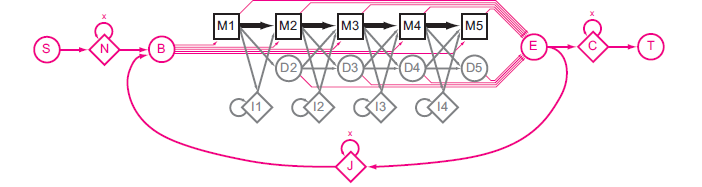
\includegraphics[width=150mm]{Figures/pHMM.png}
	\caption{Profile HMM architecture used by HMMER\citep{HMMER3}.}
	\label{fig:pHMM}
\end{figure}

Begin at Start(S), and follow some chain of arrows until arriving at Termination(T). Each arrow transits to a state of the system. 
At each state, an action can be taken either as (1) emitting a residue\footnote{In this thesis, \emph{residue} is used to refer to amino acids for protein or to nucleotides for DNA/RNA.}, or (2) selecting an arrow to the next state. The action and the selection of successor state are governed by sets of probabilities\citep{IntroBio}.
The linear core model has five sets of match (M), insertion (I) and deletion (D) states. Each M state represents one consensus position and a set of M, I, D states is the main element of the model and is referred to as a “node” in HMMER. Additional flanking states (marked as N, C, and J) emit zero or more residues from the background distribution, modelling nonhomologous regions preceding, following, or joining homologous regions aligned to the core model. Start (S), begin (B), end (E) and termination (T) states are non-emitting states.


A profile HMM for a protein family can be used to compare with query sequences, and classify sequences that are members of the family and those which are not\citep{ProteinBio}. 
A common application of profile HMMs is used to search a profile HMM against a sequence database. Another application is the query of a single protein sequence of interest against a database of profile HMMs.

\subsection{Viterbi algorithm in HMMER2}

\label{ViterbiSub}

In HMMER2, both \emph{hmmsearch} and \emph{hmmpfam} rely on the same core Viterbi algorithm for their scoring function which is named as \emph{P7Viterbi} in codes.

To find whether a sequence is member of the family described by a HMM, we compare the sequence with the HMM. We use an algorithm known as Viterbi to find one path that has the maximum probability of the HMM generating the sequence. Viterbi is a dynamic programming algorithm. Let $V_{i,j}$ be the maximum probability of a path from the start state $S_i$ ending at state $S_j$ and generating the prefix $q_{1...j}$ of the query. $V_{i+1,j}$ is found by the recurrence:

\begin{equation*}
   \displaystyle V_{i+1,j} = \max_{0 \leqslant k \leqslant j-1} \big ( V_{i,k} P(k,j)P(q_{i+1} |j) \big )
\end{equation*}

% max |x| = 
%     \begin{cases}
%     \quad -x & \text{if } x < 0,\\
%     0 & \text{if } x = 0,\\
%     x & \text{if } x > 0.
%     \end{cases}
%     max = \left\{
% \begin{array}{rl}
% -x & \text{if } x < 0,\\
% 0 & \text{if } x = 0,\\
% x & \text{if } x > 0.
% \end{array} \right.

Define $a_{ij}$ as the transition probability from state $i$ to $j$ and $e_i$ as emission probability in state $i$.
Define $V_j^M(i)$ as the log-odds score of the optimal path matching subsequence $x_{1...i}$ to the submodel up to state $j$, ending with $x_i$ being emitted by \emph{match} state $M_j$. Similarly $V_j^I(i)$ is the score of the optimal path ending in $x_i$ being emitted by \emph{insertion} state $I_j$, and $V_j^D(i)$ for the optimal path ending in \emph{deletion} state $D_j$. $q_{x_i}$ is the probability of $x_i$. Then we can write the Viterbi general equation\citep{BioSeq}:

\begin{equation*}
   V_j^M(i) = \log\frac{e_{M_j}(x_i)}{q_{x_i}} + max 
   \begin{cases}
   V_{j-1}^M(i-1) + \log a_{M_{j-1}M_j}\\
   V_{j-1}^I(i-1) + \log a_{I_{j-1}M_j}\\
   V_{j-1}^D(i-1) + \log a_{D_{j-1}M_j}
   \end{cases}
\end{equation*}

\begin{equation*}
   V_j^I(i) = \log\frac{e_{I_j}(x_i)}{q_{x_i}} + max 
   \begin{cases}
   V_j^M(i-1) + \log {a}_{M_jI_j}\\
   V_j^I(i-1) + \log a_{I_jI_j}
   \end{cases} 
\end{equation*}

\begin{equation*}
   V_j^D(i) = max 
   \begin{cases}
   V_{j-1}^M(i) + \log a_{M_{j-1}D_j}\\
   V_{j-1}^D(i) + \log a_{D_{j-1}D_j}
   \end{cases}  
\end{equation*}

The efficient DP-based pseudo code of Viterbi algorithm is shown in Algorithm\ref{Viterbi} \citep{FPGA}.  The inner loop of the code contains three two dimensional matrices (M, I, D), which calculate scores of all node positions involved in the main models for each of the residue. The outer loop consists of flanking and special states calculated in the one dimensional arrays N, B, C, J, E .

\renewcommand{\thepseudonum}{\roman{pseudonum}}
\begin{pseudocode}{Viterbi}{ }
\label{Viterbi}
\COMMENT{Initialization}\\
N[0] \GETS 0; \ \  B[0] \GETS tr(N, B)\\
E[0] \GETS C[0] \GETS J[0] \GETS -\infty\\
\COMMENT{for every sequence residue i}\\
\FOR i \GETS 1 \TO n \DO
\BEGIN
  N[i] \GETS N[i-1] + tr(N, N)\\
  B[i] \GETS max 
  \begin{cases}
   N[i-1] + tr(N, B)\\
   J[i-1] + tr(J, B)
  \end{cases}\\
  M[i,0] \GETS I[i,0] \GETS D[i,0] \GETS -\infty\\
  \COMMENT{For every model position j from 1 to m}\\
  \FOR j \GETS 1 \TO m \DO
  \BEGIN
    M[0, j] \GETS I[0, j] \GETS D[0, j] \GETS -\infty\\
    M[i, j] \GETS e(M_j, S[i]) + max 
    \begin{cases}
     M[i-1, j-1] + tr(M_{j-1}, M_j)\\
     I[i-1, j-1] + tr(I_{j-1}, M_j)\\
     D[i-1, j-1] + tr(D_{j-1}, M_j)\\
     B[i-1] + tr(B, M_j)
    \end{cases}\\
    I[i, j] \GETS e(I_j, S[i]) + max
    \begin{cases}
     M[i-1, j] + tr(M_j, I_j)\\
     I[i-1, j] + tr(I_j, I_j)
    \end{cases}\\
    D[i, j] \GETS max
    \begin{cases}
     M[i, j-1] + tr(M_{j-1}, D_j)\\
     D[i, j-1] + tr(D_{j-1}, D_j)
    \end{cases}\\
  \END\\
  E[i] \GETS max\{M[i,j] + tr(M_j, E)\} \ \  (j \GETS 0 \TO m-1)\\
  J[i] \GETS max 
  \begin{cases}
   J[i-1] + tr(J, J)\\
   E[i-1] + tr(E, J)
  \end{cases}\\
  C[i] \GETS max
  \begin{cases}
   C[i-1] + tr(C, C)\\
   E[i-1] + tr(E, C)
  \end{cases}\\
\END\\
\COMMENT{Termination: }\\
\RETURN {T(S,M) \GETS C[n] + tr(C,T)}
\end{pseudocode}

\subsection{MSV algorithm in HMMER3}

\label{MSVsub}

HMMER3 is near rewrite of the earlier HMMER2 package, with the aim of improving the speed of profile HMM searches. The main performance gain is due to a heuristic algorithm called MSV filter, for Multiple (local, ungapped) Segment Viterbi. MSV is implemented in SIMD(Single-Instruction Multiple-Data) vector parallelization instructions and is about 100-fold faster than HMMER2.

\begin{figure}[!htb]
	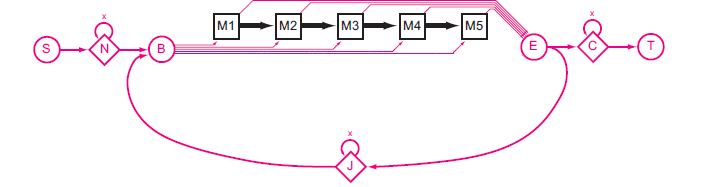
\includegraphics[width=150mm]{Figures/pHMM_msv.png}
	\caption{MSV profile: multiple ungapped local alignment segments\citep{HMMER3}.}
	\label{fig:pMSV}
\end{figure}

Figure\ref{fig:pMSV} illustrates the MSV profile architecture. Compared with Figure\ref{fig:pHMM}, the MSV corresponds to the virtual removal of the deletion and insertion states. All match-match transition probabilities are treated as 1.0. The rest parameters remains unchanged. So this model generates sequences containing one or
 more ungapped local alignment segments. The pseudo code of MSV score algorithm is simplified and shown in Algorithm\ref{MSV}.

\begin{pseudocode}{MSV}{ }
\label{MSV}
\COMMENT{Initialization}\\
N[0] \GETS 0; \ \  B[0] \GETS tr(N, B)\\
E[0] \GETS C[0] \GETS J[0] \GETS -\infty\\
\COMMENT{for every sequence residue i}\\
\FOR i \GETS 1 \TO n \DO
\BEGIN
  N[i] \GETS N[i-1] + tr(N, N)\\
  B[i] \GETS max 
  \begin{cases}
   N[i-1] + tr(N, B)\\
   J[i-1] + tr(J, B)
  \end{cases}\\
  M[i,0] \GETS -\infty\\
  \COMMENT{For every model position j from 1 to m}\\
  \FOR j \GETS 1 \TO m \DO
  \BEGIN
    M[0, j] \GETS -\infty\\
    M[i, j] \GETS e(M_j, S[i]) + max 
    \begin{cases}
     M[i-1, j-1]\\
     B[i-1] + tr(B, M_j)
    \end{cases}\\
  \END\\
  E[i] \GETS max\{M[i,j] + tr(M_j, E)\} \ \  (j \GETS 0 \TO m-1)\\
  J[i] \GETS max 
  \begin{cases}
   J[i-1] + tr(J, J)\\
   E[i-1] + tr(E, J)
  \end{cases}\\
  C[i] \GETS max
  \begin{cases}
   C[i-1] + tr(C, C)\\
   E[i-1] + tr(E, C)
  \end{cases}\\
\END\\
\COMMENT{Termination: }\\
\RETURN {T(S,M) \GETS C[n] + tr(C,T)}
\end{pseudocode}

\subsubsection*{SIMD vector parallelization in HMMER3}
\label{SSE2}

Single-Instruction Multiple-Data (SIMD) instruction is able to perform the same operation on multiple pieces of data in parallel. The SIMD vector instruction sets use 128-bit vector registers to compute up to 16 simultaneous operations. Several SIMD vector parallelization methods have been described for accelerating Smith-waterman dynamic programming. Rognes and Seeberg \citep{SW-SIMD} presented an implementation of the Smith–Waterman algorithm running on the Intel Pentium processor using the MMX SIMD instructions. A six-fold speedup was reported over an optimized non-SIMD implementation. Farrar \citep{SW-SSE2} presented an efficient vector-parallel approach called striped Smith-Waterman using Intel Streaming SIMD Extensions 2 (SSE2). A speedup of 2–8 times was reported over the Rognes and Seeberg SIMD implementations.

Similarly, since the MSV model removes deletion and insertion states that interfere with vector parallelism, the striped vector-parallel technique can be remarkably efficient way to calculate MSV alignment scores. To maximize parallelism, in HMMER3\citep{HMMER3}, Sean R. Eddy implemented MSV as a 16-fold parallel calculation with score values stored as 8-bit byte integers. He used SSE2 instructions on Intel-compatible systems and Altivec/VMX instructions on PowerPC systems.

Figure\ref{fig:strip} shows the stripped pattern. The query profile HMM of length $m$ is divided into vectors with equal length $v$. The vector length $v$ is equal to the number of elements being processed in the 128-bit SIMD register. MSV processes 8-bit byte integer with $v$ = 128/8 = 16. In a row-vectorized implementation, the query profile HMM is stored in the vectorized dynamic programming matrix dp. dp stores $m$ cells in $Q$ vectors which is numbered as $q = 1...Q$, where $Q = (m+v-1)/v$. Figure\ref{fig:strip} illustrates $m$ cells assigned to $Q$ vectors in a non-sequential way. For simple illustration, $v = 4, m = 14$, and $Q = 4$.

\begin{figure}[!htb]
	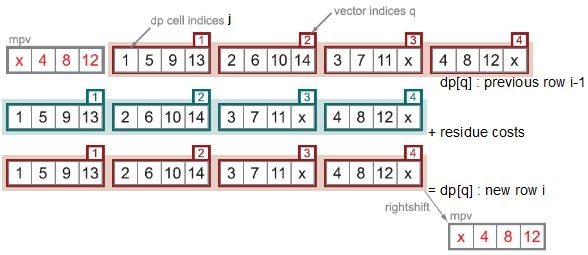
\includegraphics{Figures/msv_vector.jpg}
	\caption{Illustration of striped indexing for SIMD vector calculations\citep{HMMER3}.}
	\label{fig:strip}
\end{figure}

In Smith-Waterman and Viterbi dynamic programming, the calculation of each cell $(i, j)$ in the dp is dependent on previously calculated cells $(i-1, j), (i, j-1)$ and $(i-1, j-1)$. However, in MSV algorithm, the deletion and insertion states have been removed and only ungapped diagonals need calculating, so the calculation of each cell $(i, j)$ requires only previous $(i-1, j-1)$. In Figure\ref{fig:strip}, the top red row shows the previous row $i-1$ for the cells $j-1$, which is needed for calculating each new cell $j$ in a new row $i$. 

Striping method can remove the SIMD register data dependencies. As can be seen in the Figure\ref{fig:strip}, with striped indexing, vector $q-1$ contains exactly the four $j-1$ cells needed to calculate the four cells $j$ in a new vector $q$ on a new blue row of the dp matrix. For example, when we calculate cells $j=(2,6,10,14)$ in vector $q=2$, we access the previous row’s vector $q-1=1$ which contains the cells we need in the order we need them, $j-1=(1,5,9,13)$ (the vector above). 

\begin{figure}[!htb]
\centering
	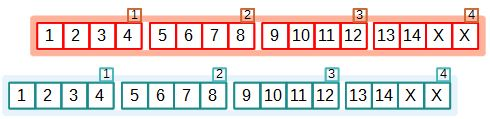
\includegraphics{Figures/msv_nostrip.jpg}
	\caption{Illustration of linear indexing for SIMD vector calculations.}
	\label{fig:nostrip}
\end{figure}

Instead, if we indexed cells into vectors in the linear order ($j=1,2,3,4$ in vector $q=1$ and so on), as shown in Figure\ref{fig:nostrip}, there is no such correspondence of $(q,q-1)$ with four $(j-1,j)$, and each calculation of a new vector $q$ would require extra expensive operations, such as shifting or rearranging cell values inside the previous row's vectors. By using the striped query access, only one shift operation is needed per row as shown in \ref{fig:strip}. Outside the inner loop(for $q = 1$ to Q), the last vector on each finished row is right-shifted (mpv, in grey with red cell $j$ indices) and used to initialize the next row calculation.

The pseudo code for the implementation is shown in Algorithm\ref{MSV-SIMD}

\begin{pseudocode}{MSV-SIMD}{ }
\label{MSV-SIMD}
\COMMENT{Initialization}\\
xJ \GETS 0; \ \  dp[q] \GETS vec\_splat(0) \  (q \GETS 0 \TO Q-1)\\
xB \GETS base + tr(N, B)\\
xBv \GETS vec\_adds(xB, tr(B, M))\\
\COMMENT{for every sequence residue i}\\
\FOR i \GETS 1 \TO n \DO
\BEGIN
  xEv \GETS vec\_splat(0)\\
  mpv \GETS vec\_rightshift(dp[Q-1])\\
  \FOR q \GETS 0 \TO Q-1 \DO
  \BEGIN
    \COMMENT{temporary  storage of 1 current row value in progress}\\
    tmpv \GETS vec\_max(mpv, xBv)\\
    tmpv \GETS vec\_adds(tmpv, e(M_j, S[i]))\\
    xEv \GETS vec\_max(xEv, tmpv)\\
    mpv \GETS dp[q]\\
    dp[q] \GETS tmpv\\
  \END\\
  xE \GETS vec\_hmax(xEv)\\
  xJ \GETS max 
  \begin{cases}
   xJ\\
   xE + tr(E, J)
  \end{cases}\\
  xB \GETS max 
  \begin{cases}
   base\\
   xJ + tr(J, B)
  \end{cases}\\
\END\\
\COMMENT{Termination: }\\
\RETURN {T(S,M) \GETS xJ + tr(C,T)}
\end{pseudocode}

Five pseudocode vector instructions for operations on 8-bit integers are used in the pseudo code. Either scalars $x$ or vectors v containing 16 8-bit integer elements numbered $v[0]...v[15]$. Each of these operations are either available or easily constructed in Intel SSE2 intrinsics as shown in the following table.

% \begin{minipage}{\textwidth}
% \begin{center}
% \begin{tabular}{|c|c|c|}\hline
% \shortstack{\textbf{Pseudocode} \\ SSE2 code in C} & \textbf{Operation} & \textbf{Definition}\\\hline
% \shortstack{\textbf{v = vec\_splat(x)} \\ v = \_mm\_set1\_epi8(x)} & assignment & $v[z] = x$\\\hline
% \shortstack{\textbf{v = vec\_adds(v1, v2)} \\ v = \_mm\_adds\_epu8(v1, v2)} & saturated addition & $v[z] = min$
% $\begin{cases}
%   2^8-1\\
%   v1[z]+v2[z]
% \end{cases}$\\\hline
% \shortstack{\textbf{v1 = vec\_rightshift(v2)} \\ v1 = \_mm\_slli\_si128(v2, 1)} & right shift & \shortstack{$v1[z] = v2[z-1](z=16...1)$; \\ $v1[0]=0;$}\\\hline
% \shortstack{\textbf{v = vec\_max(v1, v2)} \\ v = \_mm\_max\_epu8(v1, v2)} & max & $v[z] = max(v1[z], v2[z])$\\\hline
% \shortstack{\textbf{x = vec\_hmax(v)} \\ -} & horizontal max & $x = max_zv[z]$\\\hline
% \end{tabular}
% \end{center}
% \end{minipage}


\begin{table}[H]
\centering
\begin{tabular}{|c|c|c|}\hline
\shortstack{\textbf{Pseudocode} \\ SSE2 intrinsic in C} & \textbf{Operation} & \textbf{Definition}\\\hline
\shortstack{\textbf{v = vec\_splat(x)} \\ v = \_mm\_set1\_epi8(x)} & assignment & $v[z] = x$\\\hline
\shortstack{\textbf{v = vec\_adds(v1, v2)} \\ v = \_mm\_adds\_epu8(v1, v2)} & saturated addition & $v[z] = min$
$\begin{cases}
  2^8-1\\
  v1[z]+v2[z]
\end{cases}$\\\hline
\shortstack{\textbf{v1 = vec\_rightshift(v2)} \\ v1 = \_mm\_slli\_si128(v2, 1)\tablefootnote[10]{Because x86 and x86-64 use little endian, this means using a left bit shift intrinsic \_mm\_slli\_si128 to do right shift.}} & right shift & \shortstack{$v1[z] = v2[z-1](z=15...1)$; \\ $v1[0]=0;$}\\\hline
\shortstack{\textbf{v = vec\_max(v1, v2)} \\ v = \_mm\_max\_epu8(v1, v2)} & max & $v[z] = max(v1[z], v2[z])$\\\hline
\shortstack{\textbf{x = vec\_hmax(v)} \\ -\tablefootnote[11]{No SSE2 intrinsic is corresponding to vec\_hmax. Shuffle intrinsic \_mm\_shuffle\_epi32 and \_mm\_max\_epu8 can be combined to implement vec\_hmax.}} & horizontal max & $x = max(v[z]),z=0...15$\\\hline
\end{tabular}
\caption{SSE2 intrinsics for pseudocode in Algorithm\ref{MSV-SIMD}\label{tab.SSE2}}
\end{table}



%----------------------------------------------------------------------------------------
 
% % Chapter 3

\chapter{CUDA accelerated sequence alignment} % Main chapter title

\label{CUDASeqAlign} % For referencing the chapter elsewhere, use \ref{Chapter1} 

\lhead{Chapter 3. \emph{Dynamic programming in Bioinformatics}} % This is for the header on each page - perhaps a shortened title

%----------------------------------------------------------------------------------------

\section{Overview of CUDA-enabled GPU hardware}


OpenCL™ (Open Computing Language) is the first truly open and royalty-free programming standard for general-purpose computations on heterogeneous systems \citep{OpenCL}. OpenCL™ is maintained by the non-profit technology consortium Khronos Group. It has been adopted by many corporations, including Nvidia, Apple, Intel, Qualcomm, AMD, Altera, Samsung, Vivante and ARM Holdings.

Microsoft Compute Shader\citep{Shader}, also known as  DirectCompute technology, is used for GPU computing and supported on NVIDIA’s DX10 and DX11 class GPUs under Windows VISTA and later versions of Windows\citep{DirectCompute}. Compute Shader is designed and implemented with HLSL(High Level Shading Language)\citep{HLSL}, providing memory sharing and thread synchronization features to allow more effective parallel programming methods.

%----------------------------------------------------------------------------------------

\section{Overview of CUDA programming model}



%----------------------------------------------------------------------------------------

\section{CUDA accelerated Smith-Waterman}

%----------------------------------------------------------------------------------------

\section{CUDA accelerated HMMER}

%----------------------------------------------------------------------------------------

% Chapter 4

\chapter{A CUDA accelerated HMMER3 protein sequence search tool} % Main chapter title

\label{CUDAHMMER3} % For referencing the chapter elsewhere, use \ref{Chapter1} 

\lhead{Chapter \ref{CUDAHMMER3}. \emph{A CUDA accelerated HMMER3 protein sequence search tool}} % This is for the header on each page - perhaps a shortened title

%----------------------------------------------------------------------------------------

\section{Requirements and design decisions}

The following are the requirements for a CUDA accelerated HMMER3 protein sequence search tool:

\begin{itemize}
\item A HMMER3 protein sequence search tool, named cudaHmmsearch, will be implemented to run on CUDA-enabled GPU and several optimization will be taken to accelerate the computation. The cudaHmmsearch will be tested and compared with other CPU and GPU implementations.
\item The cudaHmmsearch will be based on HMMER3 algorithm so that the result will be same as hmmsearch of HMMER3.
\item The cudaHmmsearch will be completely usable under various GPU devices and sequence database size. This means that cudaHmmsearch is not just for research purpose or just a proof of concept.
\end{itemize}

\subsubsection*{Implementation toolkit and language}

NVIDIA CUDA \citep{CUDAzone} was chosen as the toolkit to be used in the implementation phase. Since its introduction in 2006, CUDA has been widely deployed through thousands of applications and published research papers, and supported by an installed base of over 500 million CUDA-enabled GPUs in notebooks, workstations, compute clusters and supercomputers \citep{CUDAwhat}. As of writing, CUDA is the most mature and popular GPU programming toolkit. 

HMMER3 is implemented in C programming language. CUDA provides a comprehensive development environment for C and C++ developers. However, some advanced features of CUDA, such as texture, are only supported in C++ template programming. So C++ has to be used, and some compatible problems when compiling and programming between C and C++ have also to be dealt with accordingly.

\subsubsection*{Implementation methods}
\label{impl}

The following two approaches have been explored for parallelizing the protein sequence database search using CUDA. A target sequence in the database is processed as one task.

\begin{itemize}
 \item \textbf{Task-based parallelism} Each task is assigned to exactly one thread, and \emph{dimBlock} tasks are performed in parallel by different threads in a thread block.
 \item \textbf{Data-based parallelism} Each task is assigned to one thread block and all \emph{dimBlock} threads in the thread block cooperate to perform the task in parallel.
\end{itemize}

Task-based parallelism has some advantages over data-based parallelism. On one side, it removes the need for inter-thread communications or, even worse, inter-multiprocessor communications. As described before, the thread or processing elements of one CUDA multiprocessor can communicate by using shared memory, while slow global memory must be used to transfer data between multiprocessors. At the same time, data-based also needs to take time on synchronizing and cooperating among threads. On the other side, to task-based, performing one sequence on each thread results in a kernel where each processing element is doing the exact same thing independently. This also simplifies implementation and testing. Although task-based parallelism needs more device memory than data-based, it can achieve better performance \citep{SW++}. Thus, the approach of task-based parallelism is taken and more efforts are put on optimizing CUDA kernel execution.

Since data-based parallelism occupies significantly less device memory, \citep{SW++} uses it to support longest query/subject sequences. However, different strategy here is applied to work around this problem and is discussed in details in subsection\ref{workload} on workload distribution.

%----------------------------------------------------------------------------------------

\section{A straightforward implementation}

This section describes a straightforward, mostly un-optimized implementation of the protein database search tool. First, a simple serial CPU implementation of hmmsearch is presented, with no GPU specific traits. Next, the MSV filter is ported to the GPU. This implementation is then optimized in the next section.

\subsection{CPU serial version of hmmsearch}

The CPU serial version of hmmsearch in HMMER3 is shown in Figure\ref{fig:hmmsearch}. The MSV and Viterbi algorithms described in subsection \ref{ViterbiSub} and \ref{MSVsub} are implemented in the so-called “acceleration pipeline” at the core of the HMMER3 software package \citep{HMMER3}. One call to the acceleration pipeline is executed for the comparison of each query model and target sequence.

\begin{figure}[!htb]
 \centering
 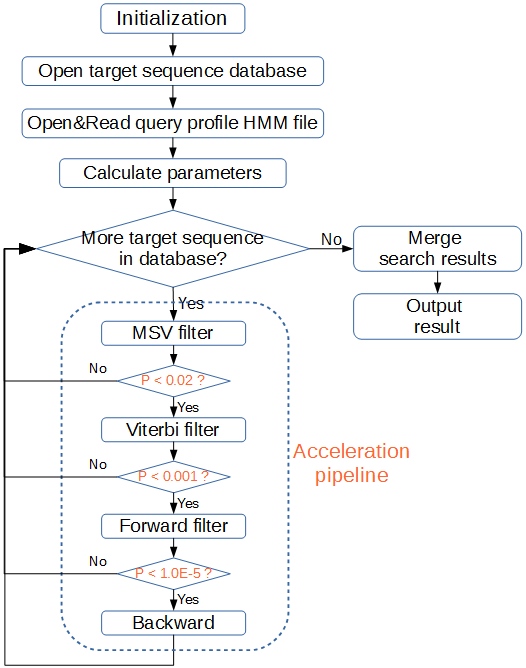
\includegraphics[totalheight=0.5\textheight]{Figures/hmmsearch.png}
 \caption{\fontfamily{pag}\selectfont The CPU serial version of hmmsearch}
 \label{fig:hmmsearch}
\end{figure}

\label{hmmsearch}
After each filter step, the pipeline either accepts or rejects the entire comparison, based on the P-value of the score calculated in each filter. For example, as can be seen in Figure\ref{fig:hmmsearch}, by default a target sequence can pass the MSV filter if its comparison gets a P-value of less than 0.02, which means the top-scoring 2\% of target sequences are expected to pass the filter. So, much fewer target sequence can pass one filter and need further computing. By this way, the comparison is accelerated. Thus, the first MSV filter is typically the run time bottleneck for hmmsearch. Therefore, the key to parallelizing hmmsearch tool is to offload the MSV filter function to multiple computing elements on GPU, while ensuring that the code shown in Figure\ref{MSV-SIMD} is as efficient as possible.

\subsection{GPU implementation of MSV filter}

A basic flow of the GPU implementation for MSV filter is shown in Figure\ref{fig:gpuMSV}. As can be seen, the code must be split up into two parts, with the left \emph{host} part running on CPU and the right \emph{device} part running on GPU. Some redundancy as data needed by GPU to compute will be copied around the memories in host and device.

\begin{figure}[!htb]
 \centering
 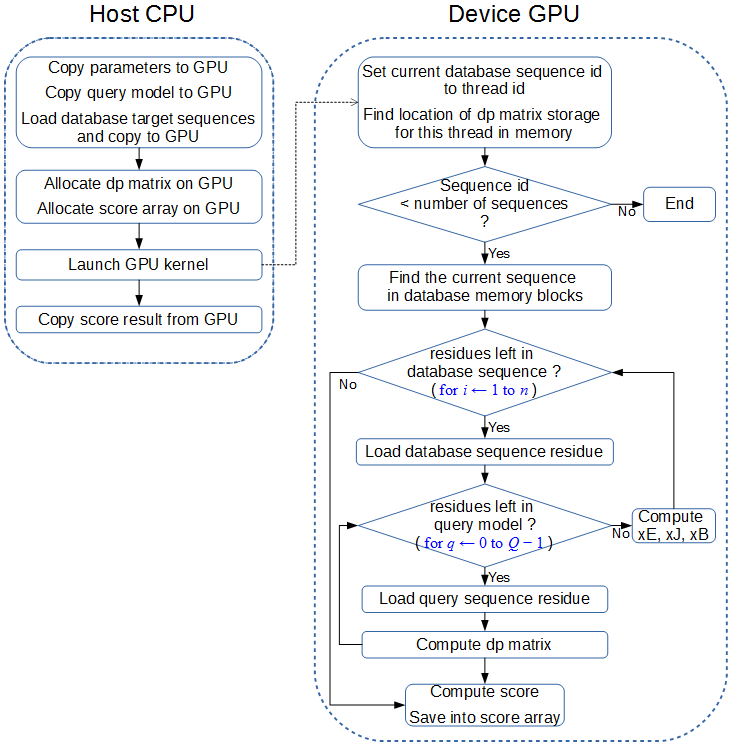
\includegraphics[totalheight=0.6\textheight]{Figures/gpuMSV.png}
 \caption{\fontfamily{pag}\selectfont The GPU porting of MSV filter}
 \label{fig:gpuMSV}
\end{figure}

The CPU code mainly concerns about allocating data structures on GPU, loading data, copying them to GPU, launching the GPU kernel and copying back the result for further steps.

The GPU kernel code is corresponding to the MSV filter Algorithm \ref{MSV-SIMD} and some more explanation are worth for it. First, the thread's current database sequence is set to the thread id. By this way each thread begins processing a different neighbouring sequence. This thread id is a unique numeric identifier for each thread and the id numbers of threads in a warp are consecutive. Next, the location where each thread can store and compute its dp matrix is determined in the global memory. This is calculated also using the thread id for each thread. When processing the sequence, successive threads access the successive addresses in the global memory for the sequence data and dp matrix, i.e. using a coalesced access pattern. Execution on GPU kernel is halted when each thread finishes its sequences.

%----------------------------------------------------------------------------------------

\section{Optimizing the implementation}

Although a fully functioning GPU MSV filter has been presented, its simple implementation is quite slow: more than 227 seconds to search a test database with 540,958 query sequences.

This section discusses the optimization steps taken to eventually reach a benchmark database search time of 1.55 seconds: an almost 147 times speedup.

\subsection{Global Memory Accesses}
\label{global}

The global memory is used to store most of data on GPU. A primary in the optimization is to improve the efficiency of accessing global memory as much as possible. One way of course is to reduce the frequency of access. Another way is coalescing access.

\subsubsection*{Access frequency}

The elements of the \emph{dp} matrix and the query profile 2D matrix are 8-bit value.  The \emph{uint4} and \emph{ulong2} (see the code below) are 128-bit CUDA built-in vector types. So the access frequency would be decreased 16 times by using \emph{uint4} or \emph{ulong2} to fetch the 8-bit value residing in global memory, compared with using 8-bit \emph{char} type.

\begin{quote}
\fontfamily{phv}\fontseries{m}\selectfont
struct \_\_device\_builtin\_\_ uint4\\
\{\\
   unsigned int x, y, z, w;\\
\}\\
struct \_\_device\_builtin\_\_ ulong2\\
\{\\
    unsigned long int x, y;\\
\};\\
\end{quote}
% \newcommand\codeHighlight[1]{\textcolor[rgb]{0,0,1}{\textbf{#1}}}
% \begin{Verbatim}[commandchars=\\\{\}]
% \codeHighlight{struct}  __device_builtin__ uint4
% \{
%     unsigned int x, y, z, w;
% \}
% \codeHighlight{struct} __device_builtin__ ulong2
% \{
%     unsigned long int x, y;
% \};
% \end{Verbatim}

This approach resulted in increased register pressure and gained a huge speed boost of almost 8 times in total.

\subsubsection*{coalescing access}

Coalescing access is the single most important performance consideration in programming for CUDA-enabled GPU architectures. Coalescing is a technique applied to combine non-contiguous and small reads/writes of global memory, into the single and more efficient contiguous and large memory reads. A prerequisite for coalescing is that the words accessed by all threads in a warp must lie in the same segment. As can be seen in Figure\ref{fig:coalescing}, the memory spaces referred to by the same variable names (not referring to same addresses) for all threads in a warp have to be allocated in the form of an array to keep them contiguous in address.

\begin{figure}[!htb]
	\centering
	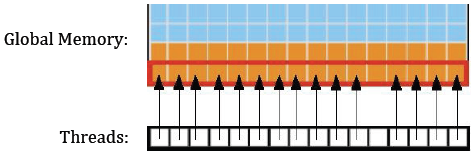
\includegraphics[totalheight=0.115\textheight]{Figures/coalesce.png}
	\caption{\fontfamily{pag}\selectfont Coalescing Global Memory Accesses\citep{Waters}.}
	\label{fig:coalescing}
\end{figure}

For coalescing access, the target sequences are arranged in an array like an upside-down bookcase shown in Figure\ref{fig:dbalign}, where all residues of a sequence are restricted to be stored in the same column from top to bottom. And all sequences are arranged in decreasing length order from left to right in the array, which is explained in section x. 

\begin{figure}[!htb]
	\centering
	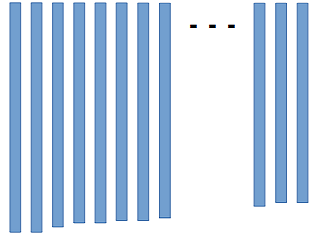
\includegraphics[totalheight=0.2\textheight]{Figures/dbalign.png}
	\caption{\fontfamily{pag}\selectfont Alignment of target sequences.}
	\label{fig:dbalign}
\end{figure}

Figure\ref{fig:dp} presents the similar global memory allocation pattern of \emph{dp} matrix for \emph{M} processing target sequences. Each thread processes independent \emph{dp} array with the same length \emph{Q}. A memory slot is allocated to a thread and is indexed top-to-bottom, and the access to \emph{dp} arrays is coalesced by using the same index for all threads in a warp.

\begin{figure}[!htb]
	\centering
	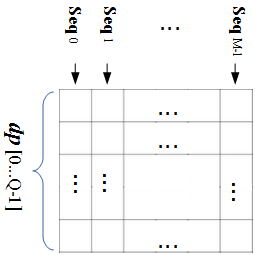
\includegraphics[totalheight=0.2\textheight]{Figures/dp.png}
	\caption{\fontfamily{pag}\selectfont The dp matrix in global memory.}
	\label{fig:dp}
\end{figure}

An alignment requirement is needed to fulfill for fully coalescing, which means any access to data residing in global memory is compiled to a single global memory instruction. The alignment requirement is automatically fulfilled for the built-in types like \emph{uint4} \citep{CUDA-C}.

The move to vertical alignment of \emph{dp} matrix resulted in an improvement of about 44\%.

\subsubsection*{Note on coding global memory coalescing access}
At the beginning, the traditional C/C++ memory block copy function \emph{memcpy}() was used, since uint4 is 16-bytes block. \emph{dp} is the pointer to the address of global memory. \emph{mpv} and \emph{sv} are \emph{uint4} data residing in register memory.

\begin{quote}
\fontfamily{phv}\fontseries{m}\selectfont
 memcpy(\&mpv, dp, sizeof(uint4));\\
 memcpy(dp, \&sv, sizeof(uint4));
\end{quote}

However, in practice of CUDA kernel execution, the above \emph{memcpy} involves 16 (sizeof(uint4)) reads and writes respectively. This does not fully coalesce access global memory. Switching to the following direct assignment resulted in 81\% improvement.

\begin{quote}
\fontfamily{phv}\fontseries{m}\selectfont
 mpv = *(dp);\\
 *(dp) = sv;
\end{quote}

\subsection{texture memory}
\label{tex}

The read-only texture memory space is a cached window into global memory that offers much lower latency and does not require coalescing for best performance. Therefore, a texture fetch costs one device memory read only on a cache miss; otherwise, it just costs one read from the texture cache. The texture cache is optimized for 2D spatial locality, so threads of the same warp that read texture addresses that are close together will achieve best performance \citep{CUDA-C}.

Texture memory is well suited to random access. CUDA has optimized the operation fetching four values (RGB colors and alpha component, a typical graphics usage) at a time in texture memory. And this mechanism is also applied to fetch four values from the query profile 2D matrix with the \emph{uint4} built-in type. Since the data of target sequences is read-only, it can also use texture for better performance.

Switching to texture memory for the query profile texOMrbv resulted in about 22\% performance improvement.

\subsubsection*{Restrictions using texture memory}

Texture memory come from the GPU graphics and therefore are less flexible than the CUDA standard types. It must be declared at compile time as a fixed type, \emph{uint4} for the query profile in our case:

\begin{quote}
\fontfamily{phv}\fontseries{mc}\selectfont
 texture$<$uint4, cudaTextureType2D, cudaReadModeElementType$>$ \emph{texOMrbv};
\end{quote}

How the values are interpreted is specified at run time. Texture memory is read-only to CUDA kernel and must be explicitly accessed via a special texture API (e.g. tex2D(), tex1Dfetch(), etc) and arrays bound to textures.

\begin{quote}
\fontfamily{phv}\fontseries{m}\selectfont
 uint4 rsc4 = tex2D(texOMrbv, x, y);
\end{quote}

However, on the CUDA next-generation architecture Kepler, the texture cache gets a special compute path, removing the complexity associated with programming it \citep{Kepler}.

\subsection{Virtualized SIMD vector programming model}

Inspired by the fact that CUDA has optimized the operation fetching a four component RGBA colour in texture memory, the target sequences is re-organized using a packed data format, where four consecutive residues of each sequence are packed together and represented using the \emph{uchar4} vector data type, instead of the \emph{char} scalar data type, as can be seen in Figure\ref{fig:simdvector}(\textit{a}). In this way, four residues are loaded using only one texture fetch, thus significantly improving texture memory throughput. 

\begin{figure}[!htb]
	\centering
	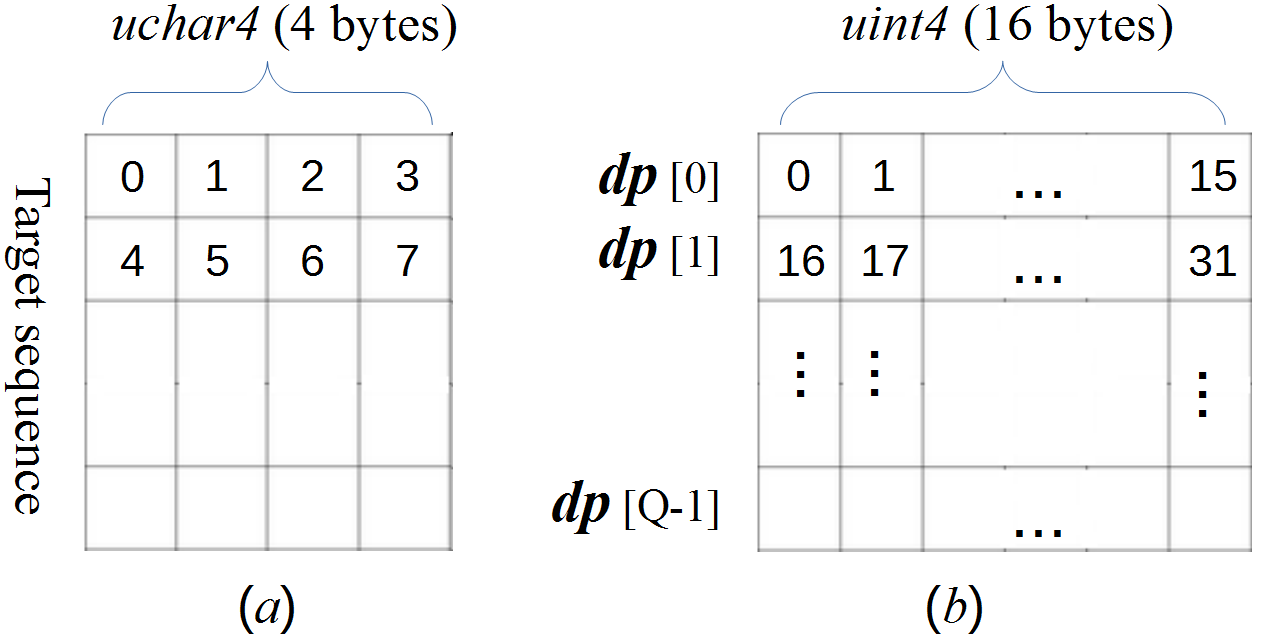
\includegraphics[totalheight=0.2\textheight]{Figures/simdvector.png}
	\caption{\fontfamily{pag}\selectfont SIMD vector alignment of data: (\textit{a}) target sequence; (\textit{b}) dp array.}
	\label{fig:simdvector}
\end{figure}

Similarly, the dp array and the query profile also use the virtualized SIMD vector allocation pattern, as can be seen in Figure\ref{fig:simdvector}(\textit{b}).

\subsection{SIMD Video Instructions}
\label{video}

Like Interl SSE2 described in subsection\ref{SSE2}, CUDA also provides the scalar SIMD (Single Instruction, Multiple Data) video instructions. These are available on devices of compute capability 3.0. The SIMD video instructions enable efficient operations on pairs of 16-bit values and quads of 8-bit values needed for video processing.

The SIMD video instructions can be included in CUDA programs by way of the assembler, \emph{asm}(), statement.

The basic syntax of an \emph{asm}() statement is:

\begin{quote}
\fontfamily{phv}\fontseries{m}\selectfont
 asm(``template-string" : ``constraint''(output) : ``constraint"(input));
\end{quote}

The following three instructions are used in the implementation. Every instruction operates on quads of 8-bit signed values. The source operands(“op1” and “op2”) and destination operand(“rv”) are all unsigned 32-bit registers(“u32”), which is different from 128-bit in SSE2. For additions and subtractions, saturation instructions(“sat”) have been used to clamp the values to their appropriate unsigned ranges.

\begin{quote}
\fontfamily{phv}\fontseries{mc}\selectfont
 \textsl{/* rv[z] = op1[z] + op2[z] (z = 0,1,2,3) */}\\
 asm(``vadd4.u32.u32.u32.sat \%0, \%1, \%2, \%3;" : ``=r"(rv) : ``r"(op1), ``r"(op2), ``r"(0));\\
 \textsl{/* rv = op1 + op2 */}\\
 asm(``vsub4.u32.u32.u32.sat \%0, \%1, \%2, \%3;" : ``=r"(rv) : ``r"(op1), ``r"(op2), ``r"(0));\\
 \textsl{/* rv = max(op1,op2) */}\\
 asm(``vmax4.u32.u32.u32 \%0, \%1, \%2, \%3;" : ``=r"(rv) : ``r"(op1), ``r"(op2), ``r"(0));
% \slshape A narrow slanted f\'ee.\\
\end{quote}

Switching to the SIMD video instructions also achieved a large speedup of nearly 2 times.

\subsection{Pinned (non-pageable) Memory}
\label{pin}

It is necessary to transfer data to the GPU over the PCI-E data bus. Compared to access to CPU host memory, this bus is very slow. Pinned memory is memory that cannot be paged (swapped) out to disk by the virtual memory management of the OS. In fact, PCI-E transfer can only be done using pinned memory, and if the application does not allocate pinned memory, the CUDA driver does this in the background for us. Unfortunately, this results in a needless copy operation from the regular (paged) memory to or from pinned memory. We can of course eliminate this by allocating pinned memory ourselves.

In the application, we simply replace \emph{malloc/free} when allocating/freeing memory in the host application with \emph{cudaHostAlloc/cudaFreeHost}.

\begin{quote}
\fontfamily{phv}\fontseries{m}\selectfont
 cudaHostAlloc (void** host\_pointer, size\_t size, unsigned int flags)
\end{quote}

\subsection{Asynchronous memory copy and Streams}
\label{asyn}

\subsubsection*{Asynchronous memory copy}
By default, any memory copy involving host memory is synchronous: the function does not return until after the operation has been completed. This is because the hardware cannot directly access host memory unless it has been page-locked or pinned and mapped for the GPU. An asynchronous memory copy for pageable memory could be implemented by spawning another CPU thread, but so far, CUDA has chosen to avoid that additional complexity.

Even when operating on pinned memory, such as memory allocated with \emph{cudaMallocHost}(), synchronous memory copy must wait until the operation is finished because the application may rely on that behavior. When pinned memory is specified to a synchronous memory copy routine, the driver does take advantage by having the hardware use DMA, which is generally faster \citep{CUDAHand}.

When possible, synchronous memory copy should be avoided for performance reasons. Keeping all operations asynchronous improves performance by enabling the CPU and GPU to run concurrently. Asynchronous memory copy functions have the suffix \emph{Async}(). For example, the CUDA runtime function for asynchronous host to device memory copy is \emph{cudaMemcpyAsync}().

It works well only where either the input or output of the GPU workload is small in comparison to one another and the total transfer time is less than the kernel execution time. By this means we have the opportunity to hide the input transfer time and only suffer the output transfer time.

\subsubsection*{Multiple streams}
A CUDA stream represents a queue of GPU operations that get executed in a specific order. We can add operations such as kernel launches, memory copies, and event starts and stops into a stream. The order in which operations are added to the stream specifies the order in which they will be executed. CUDA streams enable CPU/GPU and memory copy/kernel processing concurrency. For GPUs that have one or more copy engines, host $\longleftrightarrow$ device memory copy can be performed while the SMs are processing kernels. Within a given stream, operations are performed in sequential order, but operations in different streams may be performed in parallel \citep{CUDAintro}.

To take advantage of CPU/GPU concurrency as depicted in Figure\ref{fig:cpu_gpu}, when performing memory copies as well as kernel launches, asynchronous memory copy must be used. And Mapped pinned memory can be used to overlap PCI Express transfers and kernel processing.

\begin{figure}[!htb]
	\centering
	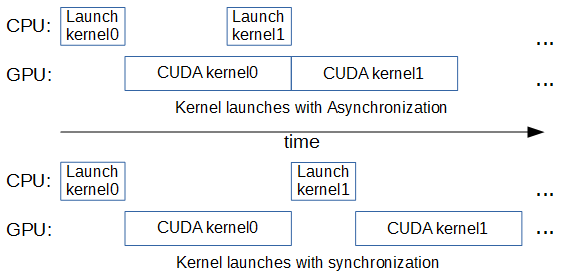
\includegraphics[totalheight=0.3\textwidth]{Figures/cpu_gpu.png}
	\caption{\fontfamily{pag}\selectfont CPU/GPU concurrency.}
	\label{fig:cpu_gpu}
\end{figure}

CUDA compute capabilities above 2.0 are capable of concurrently running multiple kernels, provided they are launched in different streams and have block sizes that are small enough so a single kernel will not fill the whole GPU.

By using multiple streams, we broke the kernel computation into chunks and overlap the memory copies with kernel execution. The new improved implementation might have the execution timeline as shown in Figure\ref{fig:streams} in which empty boxes represent time when one stream is waiting to execute an operation that it cannot overlap with the other stream's operation.

\begin{figure}[!htb]
	\centering
	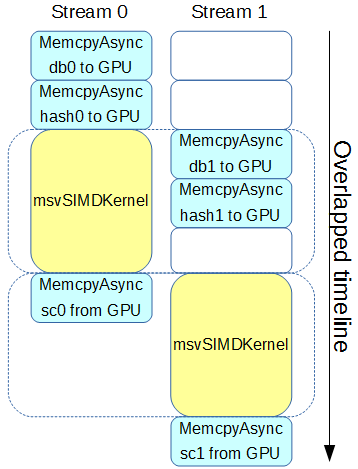
\includegraphics[totalheight=0.32\textheight]{Figures/streams.png}
	\caption{\fontfamily{pag}\selectfont Timeline of intended application execution using two independent streams.}
	\label{fig:streams}
\end{figure}
% \begin{lstlisting}[language=C++, caption={Combined asynchronous memory copy and multiple streams}, captionpos=t]
% // enqueue copies of dbQuad in stream0 and stream1
% cudaMemcpyAsync(cudaPtr.dbQuad0, hostPtr.dbQuad0,
% 		num0 * sizeof(uint),
% 		cudaMemcpyHostToDevice,
% 		stream[0]);
% cudaMemcpyAsync(cudaPtr.dbQuad1, hostPtr.dbQuad1,
% 		num2 * sizeof(uint),
% 		cudaMemcpyHostToDevice,
% 		stream[1]);
% 
% // enqueue copies of hashQuad in stream0 and stream1
% cudaMemcpyAsync(cudaPtr.hashQuad0, hostPtr.hashQuad0, num0 * sizeof(uint), cudaMemcpyHostToDevice, stream[0]);
% cudaMemcpyAsync(cudaPtr.hashQuad1, hostPtr.hashQuad1, num1 * sizeof(uint), cudaMemcpyHostToDevice, stream[1]);
% 
% // enqueue kernels in stream0 and stream1
% msvSIMDKernel0<<<numBlocks, KERNEL_BLOCKSIZE, 0, stream[0]>>>();
% msvSIMDKernel0<<<numBlocks, KERNEL_BLOCKSIZE, 0, stream[1]>>>();
% 
% // enqueue copies of result from device to locked memory
% cudaMemcpyAsync(hostSC0, cudaSC0, num0 * sizeof(float), cudaMemcpyDeviceToHost, stream[0]);
% cudaMemcpyAsync(hostSC1, cudaSC1, num1 * sizeof(float), cudaMemcpyDeviceToHost, stream[1]);
% \end{lstlisting}

Running the improved program using pinned memory, asynchronous memory copy and two streams reveals the time drops from 16.45s to just 9.46s, a quite significant drop of over 73.8\% in execution time.

\subsection{Sorting database}
\label{dbsort}
As described in Section\ref{MSVsub}, MSV filter function is sensitive to the length of a target sequence, which determines the execution times of main \emph{for} loop in Algorithm\ref{MSV-SIMD}. 

Target sequence database could contain many sequences with different lengths.  The 24GB NCBI NR database consists of over 38 million sequences with sequence lengths varying from 6 $\sim$ 37,000+ amino acids \citep{NCBI}.

This brings a problem for parallel processing of threads on GPU: one thread could be processing a sequence of several thousands of residues while another might be working on a sequence of just a few. As a result, the thread that finishes first might be idle while the long sequence is being handled. Furthermore, unless care is taken when assigning sequences to threads, this effect might be compounded by the heavily unbalanced workload among threads.

In order to achieve high efficiency for task-based parallelism, the run time of all threads in a thread block should be roughly identical. Therefore the database is converted with sequences being sorted by length. Thus, for two adjacent threads in a thread warp, the difference value between the lengths of the associated sequences is minimized, thereby balancing a similar workload over threads in a warp.

\subsubsection*{Block reading}
Many research implementation were not concerned with practical matters. They just loaded the whole database data into memories of CPU host and GPU device. Large database, like NCBI NR database, is more than 24GB in size and is still increasing, being too large to load into memories of most machines.

Given GPU global memory is much less than CPU host, we use the size of GPU global memory as the basis to decide the size of sequence block while reading the database.

\subsubsection*{Descending order}
The memory pools for database sequences both in CPU host and GPU device are dynamically allocated at run time. The pools may be required to reallocated due to more space needed for the current data block than the last one. If the pool allocated at the first time is the largest one during execution, then the overhead of reallocation will be saved. Hence, the descending order is used for sorting the database.

\subsubsection*{Performance improved}
The CUDA profiling tool nvprof \citep{Profiler} was used to understand and optimize the performance of the MSV GPU application cudaHmmsearch. The nvprof command was used as follows:

\begin{quote}
\fontfamily{phv}\fontseries{m}\selectfont
 \# nvprof  ./cudaHmmsearch globins4.hmm uniprot\_sprot.fasta
\end{quote}

The table\ref{tab.nvprof1} and \ref{tab.nvprof2} list the profiling results of before and after the target database was sorted.

\begin{table}[H]
\centering
\begin{tabular}{|c|c|c|c|c|c|c|}\hline
\shortstack{\textbf{Time(\%)}} & \shortstack{\textbf{Time}} & \shortstack{\textbf{Calls}} & \shortstack{\textbf{Avg}} & \shortstack{\textbf{Min}} & \shortstack{\textbf{Max}} & \shortstack{\textbf{Name}} \\\hline
91.61\% & 4.27108s & 134 & 31.874ms & 5.9307ms & 137.67ms & msvSIMDKernel\\\hline
8.37\% & 390.01ms & 271 & 1.4391ms & 704ns& 23.027ms& [CUDA memcpy HtoD]\\\hline
0.01\% & 556.21us & 134 & 4.1500us & 1.7280us & 5.9840us& [CUDA memcpy DtoH]\\\hline
0.01\% & 491.23us & 134 & 3.6650us & 3.4880us& 4.0640us& [CUDA memset]\\\hline
\end{tabular}
\caption{\fontfamily{pag}\selectfont\textbf{Profiling result of before sorting database.} Each row is the statistics of profiling result for the function named in the `\textbf{Name}'. The statistics includes the percentage of running time, the running time, the number of called times, as well as the average, minimum, and maximum time.\label{tab.nvprof1}}
\end{table}

\begin{table}[H]
\centering
\begin{tabular}{|c|c|c|c|c|c|c|}\hline
\shortstack{\textbf{Time(\%)}} & \shortstack{\textbf{Time}} & \shortstack{\textbf{Calls}} & \shortstack{\textbf{Avg}} & \shortstack{\textbf{Min}} & \shortstack{\textbf{Max}} & \shortstack{\textbf{Name}} \\\hline
97.41\% & 2.07263s & 134 & 15.467ms & 29.056us & 194.91ms & msvSIMDKernel\\\hline
2.54\% & 54.115ms & 271 & 199.69us & 704ns& 23.013ms& [CUDA memcpy HtoD]\\\hline
0.03\% & 550.53us & 134 & 4.1080us & 1.6640us & 4.6720us& [CUDA memcpy DtoH]\\\hline
0.02\% & 474.90us & 134 & 3.5440us & 672ns& 4.0320us& [CUDA memset]\\\hline
\end{tabular}
\caption{\fontfamily{pag}\selectfont\textbf{Profiling result of after sorting database.} The meaning of each column is same as Table\ref{tab.nvprof1}\label{tab.nvprof2}}
\end{table}

From the result of profiling, we can see the performance has been increased, which is clearly shown in two ways:
\begin{enumerate}
 \item the ratio of the msvSIMDKernel run-time to the total increased from 91.61\% to 97.41\%;
 \item the  msvSIMDKernel run-time decreased from 4.27108s to 2.07263s and the time of the memory copy from Host to Device (CUDA memcpy HtoD) decreased from 390.01ms to 54.115ms.
\end{enumerate}

This approach has the advantage of being both effective and quite straightforward as a large 129\% performance improvement can be gained over the unsorted database without changing the GPU kernel in any way (see Table\ref{tab.opt} and Figure\ref{fig:imp}). For the 24GB NCBI NR database used in these experiments, only 6 minutes were taken for sorting. Further, the sorted database can still be usable for other applications, making the one-time cost of sorting it negligible.

\subsection{Distributing workload}
\label{workload}
After launching GPU kernel, CPU must wait for the GPU to finish before copying back the result. This is accomplished by calling \emph{cudaStreamSynchronize}( \emph{stream} ). We can get further improvement by distribute some work from GPU to CPU while CPU is waiting. In protein database, the sequences with the longest or the shortest length are very few. According to Swiss-Prot database statistics \citep{Swiss-Prot}, the percentage of sequences with length $>$ 2500 is only 0.2\%. Considering the length distribution of database sequences and based on the descending sorted database discussed in section\ref{dbsort}, we assigned the first part of data with longer lengths to CPU. By this way, we can save both the GPU global memory allocated for sequences and the overheads of memory transfer.

The compute power of CPU and GPU should be taken into consideration in order to balance the workload distribution between CPU and GPU. The distribution policy calculates a ratio \emph{R} of the number of database sequences assigned to GPU, which is calculated as

\begin{equation*}
   R = \frac{N_Gf_G}{N_Gf_G + f_C}
\end{equation*}

where $f_G$ and $f_C$ are the core frequencies of GPU and CPU, $N_G$ is the number of GPU Multiprocessors.

%----------------------------------------------------------------------------------------

\subsection{Miscellaneous consideration}
This sections discusses various small-scale optimization and explains some techniques not suited to the MSV implementation.

\subsection*{Data type for register memory}
\label{register}
In order to reduce the register pressure in CUDA kernel, we may consider using unsigned 8-bit char type (u8) instead of 32-bit int type (u32). Declaring the registers as u8 results in sections of code to shift and mask data. The extract data macros are deliberately written to mask off the bits that are not used, so this is entirely unnecessary. In fact, around four times the amount of code will be generated if using an u8 type instead of an u32 type.

Changing the u8 definition to an u32 definition benefits from eliminating huge numbers of instructions. It seems potentially wasting some register space. In practice, CUDA implements u8 registers as u32 registers, so this does not actually cost anything extra in terms of register space \citep{cook}.

\subsubsection*{Branch divergence}
\label{branch}

A warp executes one common instruction at a time, so full efficiency is realized when all 32 threads of a warp agree on their execution path. If threads of a warp diverge via a data-dependent conditional branch, the warp serially executes each branch path taken, disabling threads that are not on that path, and when all paths complete, the threads converge back to the same execution path. Branch divergence occurs only within a warp; different warps execute independently regardless of whether they are executing common or disjoint code paths. So the divergence results in some slowdown.

Since the implementation has changed u8 type in register memory to u32 type, the test for the overflow condition is not needed any more. This not only saves several instructions, but also avoids the issue of branch divergence.

\subsubsection*{Constant memory}
\label{constant}
Constant memory is as fast as reading from a register as long as all threads in a warp read the same 4-byte address. Constant memory does not support, or benefit from, coalescing, as this involves threads reading from different addresses. Thus, parameters used by all threads, such as $base$, $t_{jb}$, $t_{ec}$, are stored into constant memory.

\subsubsection*{Shared memory}
\label{shared}
In terms of speed, shared memory is perhaps 10x slower than register accesses but 10x faster than accesses to global memory. However, some disadvantages apply to shared memory.

\begin{itemize}
 \item Unlike the L1 cache, the shared memory has a per-block visibility, which would mean having to duplicate the data for every resident block on the SM.
 \item Data must be loaded from global to shared memory in GPU kernel and can not be uploaded to shared memory directly from the host memory.
 \item Shared memory is well suited to exchange data between CUDA threads within a block. As described in subsection\ref{impl}, task-based parallelism is applied without the need for inter-thread communications, which also saves the cost of synchronization \emph{\_\_syncthreads}() among threads.
\end{itemize}

Because of these disadvantages, the MSV implementation does not use shared memory.

\subsubsection*{Kernel launch configuration}
\label{launch}
Since the MSV implementation does not use shared memory explained above, the following dynamic kernel launch configuration is used to prefer larger L1 cache and smaller shared memory so as to further improve memory throughput.
\begin{quote}
\fontfamily{phv}\fontseries{m}\selectfont
 cudaFuncSetCacheConfig(msvSIMDKernel, cudaFuncCachePreferL1);
\end{quote}

%----------------------------------------------------------------------------------------

\section{Conclusion of optimization}
Summary of optimization steps taken

This section briefly reviews the all the optimization approaches discussed in this chapter thus far, and summarizes the steps to gain better performance for CUDA programming.

\subsection*{Six steps to better performance}
\begin{enumerate}
 \item Assessing the application\\
 In order to benefit from any modern processor architecture, including GPUs, the first steps are to assess the application to identify the hotspots [MSV filter in Section\ref{hmmsearch}], which type of parallelism [Task-based parallelism in Section\ref{impl}] is better suited to the application.
 \item Application Profiling\\
 NVIDIA provides profiling tools to help identify hotspots and compile a list of candidates for parallelization or optimization on CUDA-enabled GPUs [nvprof in Section\ref{dbsort}], as detailed in Section\ref{cudaTools}. 
 Intel provides VTune Amplifier XE to collect a rich set of data to tune CPU \& GPU compute performance at \url{https://software.intel.com/en-us/intel-vtune-amplifier-xe}.
 
 \item Optimizing memory usage\\
 Optimizing memory usage starts with minimizing data transfers both in size [Data-base sorted in Section\ref{dbsort}, workload distribution in Section\ref{workload}] and time [Pinned Memory in Section\ref{pin}] between the host and the device [Asynchronous memory copy in Section\ref{asyn}]. Be careful with CUDA memory hierarchy: register memory [Section\ref{register}], local memory, shared memory [Section\ref{shared}], global memory, constant memory [Section\ref{constant}] and texture memory [Section\ref{tex}], and combine these memories to best suit the application [Kernel launch configuration in Section\ref{launch}]. Sometimes, the best optimization might even be to avoid any data transfer in the first place by simply recomputing the data whenever it is needed.\\
 The next step in optimizing memory usage is to organize memory accesses according to the optimal memory access patterns. This optimization is especially important for coalescing global memory accesses [Section\ref{global}].
 
 \item Optimizing instruction usage\\
 This suggests using SIMD Video Instructions [Section\ref{video}] and trading precision for speed when it does not affect the end result, such as using intrinsic instead of regular functions or single precision instead of double precision [HMMER3 in Section\ref{SSE2}]. Particular attention should be paid to control flow instructions [Branch divergence in Section\ref{branch}].
 
 \item Maximizing parallel execution
 
 The application should maximize parallel execution at a higher level by explicitly exposing concurrent execution on the device through streams [Section\ref{asyn}], as well as maximizing concurrent execution between the CPU host  [Database sorted in Section\ref{dbsort}] and the GPU device [Workload distribution in Section\ref{workload} and SIMD Video Instructions in Section\ref{video}].
 
 \item Considering the existing libraries
 
 Many existing GPU-optimized libraries \citep{CUDAlibs} such as cuBLAS \citep{cuBLAS}, MAGMA \citep{MAGMA}, ArrayFire \citep{ArrayFire}, or Thrust \citep{thrust}, are available to make the expression of parallel code as simple as possible.
 
\end{enumerate}


 
% Chapter 5

\chapter{Benchmark results and discussion} % Main chapter title
\label{Results} % For referencing the chapter elsewhere, use \ref{Chapter1} 

\lhead{Chapter \ref{Results}. \emph{Benchmark results and discussion}} % This is for the header on each page - perhaps a shortened title

Chapter\ref{CUDAHMMER3} described several approaches to optimize the cudaHmmsearch implementation. This chapter presents the performance measurements when experimenting these approaches on a GPU and on a multicore CPU.
%----------------------------------------------------------------------------------------

\section{Benchmarking environment}
The benchmarking environment were set up in Kronos machine \label{Kronos}as follows:

\begin{itemize}
 \item CPU host\\
 Intel� Core� i7-3960X with 6 cores, 3.3GHz clock speed, 64GB RAM
 \item GPU device\\
 NVIDIA� Quadro� K4000 graphics card with 3 GB global memory, 768 Parallel-Processing Cores, 811 MHz GPU Clock rate, CUDA Compute Capability 3.0.
 \item Software system\\
 The operating system used was Ubuntu 64 bit Linux v12.10; the CUDA toolkit used was version 5.5.
 \item Target sequences database\\
 One was Swiss-Prot database in fasta format released in September 2013 \citep{UniProt} containing 540,958 sequences with length varying from 2 $\sim$ 35,213 amino acids, comprising 192,206,270 amino acids in total, more than 258MB in file size. Another was much larger NCBI NR database in fasta format released in April 2014 \citep{NCBI} containing 38,442,706 sequences with length varying from 6 $\sim$ 37,000+ amino acids, comprising 13,679,143,700 amino acids in total, more than 24GB in file size.
 \item Query profile HMMs\\
 \label{pHMMs}
 We tested 5 profile HMMs of length 149, 255, 414, 708 and 1111 states, detailed in Table\ref{tab.phmms}. Globin4 with length of 149 states was distributed with the HMMER source \citep{Hsource}. Other 4 HMMs were taken directly from the Pfam database \citep{Pfam} that vary in length from 255 to 1111 states.\\
 \begin{table}[H]
 \centering
 \begin{tabular}{|c|c|c|c|c|c|}\hline
 \textbf{Name} & Globin4 & 120\_Rick\_ant & 2HCT & ACC\_central & AAA\_27 \\\hline
 \textbf{Accession number} & - & PF12574.3 & PF03390.10 & PF08326.7 & PF13514.1 \\\hline
 Length & 149 & 255 & 414 & 708 & 1111 \\\hline
 \end{tabular}
 \caption{\fontfamily{pag}\selectfont Profile HMMs used in benchmarking. \label{tab.phmms} Globin4 has no Accession number.}
 \end{table}
 \item Measuring method\\
 The execution time of the application was timed using the C clock() instruction. The performance was measured in unit GCUPS(Giga Cell Units Per Second) which is calculated as follows:
 \begin{equation*}
   GCUPS = \frac{L_q * L_t}{T * 1.0e09}
 \end{equation*}
 where $L_q$ is the length of query profile HMM, i.e. the number of the HMM states, $L_t$ is the total residues of target sequences in the database, $T$ is the execution time in second.\\
 All programs were compiled using GNU g++ with the -O3 option and executed independently in a 100\% idle system.
\end{itemize}

%----------------------------------------------------------------------------------------

\section{Performance Results}

\subsection{Comparison with less optimized approaches}
To show the performance impact of several selected optimization approaches, the performance of the implementation was compared with that of previous approach.

Table\ref{tab.opt} shows the approaches taken in optimizing performance. All tests are taken against the Swiss-Prot database. The query HMM used was globin4. The fourth column `Improvement' is measured in percentage compared with the previous approach.

\begin{table}[H]
\centering
\begin{tabular}{|c|c|c|c|}\hline
\shortstack{\textbf{Description of} \\ \textbf{approach}} & \shortstack{\textbf{Execution} \\ \textbf{time (s)}} & \shortstack{\textbf{Performance}\\ (GCUPS)} & \shortstack{\textbf{Improvement}\\ \textbf{(\%)}}\\\hline
Initial implementation & 227.178 & 0.126 & - \\\hline
SIMD Video Instruction& 125.482 & 0.228 & 81 \\\hline
\shortstack{Minimizing global\\memory access} & 16.449 & 1.741 & 664 \\\hline
\shortstack{Async memcpy \&\\Multi streams} & 9.463 & 3.026 & 74 \\\hline
\shortstack{Coalescing of\\global memory} & 6.565 & 4.362 & 44 \\\hline
Texture memory & 5.370 & 5.333 & 22 \\\hline
Sorting Database & 2.346 & 12.207 & 129 \\\hline
Distributing workload & 1.650 & 17.357 & 42 \\\hline
\end{tabular}
\caption{\fontfamily{pag}\selectfont \textbf{Performance of optimization approaches.} The fourth column \textbf{Improvement} is measured in percentage compared with the previous approach. The row `Coalescing of global memory' is benchmarked only for the $dp$ matrix. The row `Texture memory' is benchmarked only for the query profile texOMrbv 2D texture. \label{tab.opt}}
\end{table}

The graphic view corresponding to Table is shown in Figure\ref{fig:imp}. 

\begin{figure}[!htb]
	\centering
	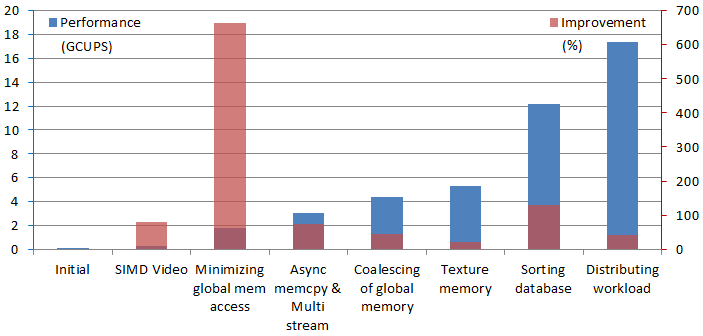
\includegraphics[totalheight=0.28\textheight]{Figures/improve.png}
	\caption{\fontfamily{pag}\selectfont \textbf{Performance of optimization approaches.} The data of this chart come from Table\ref{tab.opt}. The blue bar is Performance (in GCUPS) of each approach, corresponding to the left Y axis. The red bar is Improvement in \% corresponding to the right Y axis.}
	\label{fig:imp}
\end{figure}

From the chart, it can be seen that several factors are related to global memory accesses, including the highest 663\% minimizing global memory access, coalescing of global memory and texture memory. So the global memory optimizations are the most important area for performance. To make all threads in a warp execute similar tasks, the auxiliary sorting database also plays important role in optimizations.

\subsection{Practical benchmark}
\label{Pbench}
The final cudaHmmsearch implementation, with the optimization discussed in Chapter\ref{CUDAHMMER3}, was benchmarked to determine its real-world performance. This was done by searching the much large NCBI NR database for several profile HMMs with various lengths, as detailed in Section\ref{pHMMs}. As comparison, the same searches were executed by hmmsearch of HMMER3 on 1 CPU core.

\begin{table}[H]
\centering
\begin{tabular}{|c|c|c|c|c|c|}\hline
\shortstack{\textbf{Profile HMM} \\ \textbf{(length)}} & \shortstack{\textbf{globins4} \\ (149)} & \shortstack{\textbf{120\_Rick\_ant}\\ (255)} & \shortstack{\textbf{2HCT}\\ (414)} & \shortstack{\textbf{ACC\_central} \\ (708)} & \shortstack{\textbf{AAA\_27} \\ (1111)} \\\hline
\shortstack{Performance of \\ hmmsearch \\ (GCUPS)} & 9.37 & 11.72 & 11.68 & 11.96 & 6.90 \\\hline
\shortstack{Performance of \\ cudaHmmsearch \\ (GCUPS)} & 23.00 & 32.17 & 30.01 & 32.83 & 14.68 \\\hline
\shortstack{Speedup \\ (times)} & 2.45 & 2.74 & 2.57 & 2.75 & 2.13 \\\hline
\end{tabular}
\caption{\fontfamily{pag}\selectfont \textbf{Result of Practical benchmark.} \label{tab.pb} Speedup is measured in times of cudaHmmsearch performance over that of hmmsearch.}
\end{table}

The results of the benchmarks are shown in graphical form in Figure\ref{fig:len}. The GPU cudaHmmsearch performance hovers just above 25 GCUPS, while the CPU hmmsearch only around 10 GCUPS. The whole performance of cudaHmmsearch is stable with various lengths of query HMMs. On average, cudaHmmsearch has a speedup of 2.5x than hmmsearch. 

\begin{figure}[!htb]
	\centering
	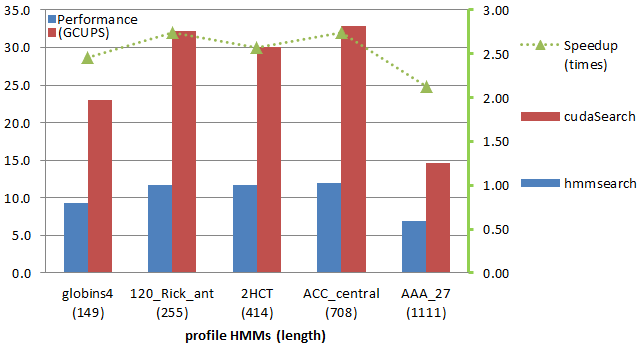
\includegraphics[totalheight=0.36\textheight]{Figures/lengths.png}
	\caption{\fontfamily{pag}\selectfont \textbf{Practical benchmarks.} The data of this chart come from Table\ref{tab.pb}. The blue and red bar is Performance (in GCUPS) of hmmsearch and cudaHmmsearch respectively, corresponding to the left Y axis. The green dot line is Speedup (in times) of cudaHmmsearch performance over that of hmmsearch, corresponding to the right Y axis.}
	\label{fig:len}
\end{figure}

Figure\ref{fig:len} shows that the performance of both GPU and CPU searching for AAA\_27 dropped greatly. The reason can be seen from the table\ref{tab.sta} listing the internal pipeline statistics summary for searching globin4 and AAA\_27. For every filter, the count of passed sequences for searching AAA\_27 with 1111 states is much more than that of globin4 with 149 states. This means that for searching AAA\_27, much more target sequences than searching globin4 are needed calculating in each filter after MSV filter. And at the same time, each filter is more time-consuming than MSV filter. All of these result in the AAA\_27 performance dropping greatly.

\begin{table}[H]
\centering
\begin{tabular}{|c|c|c|}\hline
\shortstack{\textbf{Query profile HMM(length)}} & \shortstack{\textbf{globin4 (149 states)}} & \shortstack{\textbf{AAA\_27 (1111 states)}}\\\hline
Target sequences & 38442706 & 38442706 \\\hline
Passed MSV filter & 1195043 & 4305846 \\\hline
Passed bias filter & 973354 & 1671084 \\\hline
Passed Viterbi filter & 70564 & 322206 \\\hline
Passed Forward filter & 7145 & 17719 \\\hline
\end{tabular}
\caption{\fontfamily{pag}\selectfont Internal pipeline statistics summary\label{tab.sta}}
\end{table}

\subsection{Comparison with multicore CPU}
Since multicore processors were developed in the early 2000s by Intel, AMD and others, nowadays CPU has become multicore with two cores, four cores, six cores and more. The Kronos \ref{Kronos} experiment system has CPU with six cores. This section presents the benchmarks of cudaHmmsearch running with multiple CPU cores.

The experiment was done by executing cudaHmmsearch and hmmsearch with 1, 2...6 CPU cores, searching the NCBI NR database for the HMM with 255-state length.

The benchmark has not been used in the articles cited in this thesis. The purpose of this benchmark is to show how the performance increase or decrease with more CPU cores involved in computing.

\begin{table}[H]
\centering
\begin{tabular}{|c|c|c|c|c|c|c|}\hline
\shortstack{\textbf{Performance} \\ \textbf{(GCUPS)}} & \shortstack{1 CPU \\ core} & \shortstack{2 CPU \\ cores} & \shortstack{3 CPU \\ cores} & \shortstack{4 CPU \\ cores} & \shortstack{5 CPU \\ cores} & \shortstack{6 CPU \\ cores} \\\hline
cudaHmmsearch & 32.17 & 50.22 & 57.70 & 59.14 & 59.39 & 59.29 \\\hline
hmmsearch & 11.72 & 23.28 & 29.22 & 44.15 & 46.19 & 44.69 \\\hline
\end{tabular}
\caption{\fontfamily{pag}\selectfont {Result of Comparison with multicore CPU.} \label{tab.mcpu}}
\end{table}

Figure\ref{fig:cpuCores} shows the benchmark result. The number performance results is measured in GCUPS. As can be seen, from 1 CPU core to 4 CPU cores, both cudaHmmsearch performance and hmmsearch performance go up almost linearly. From then on, due to complex schedule among CPU cores, the extra CPU core will not contribute much to both cudaHmmsearch and hmmsearch execution. Even worse, it will have negative effect as shown clearly in the `6 CPU' case.

\begin{figure}[!htb]
	\centering
	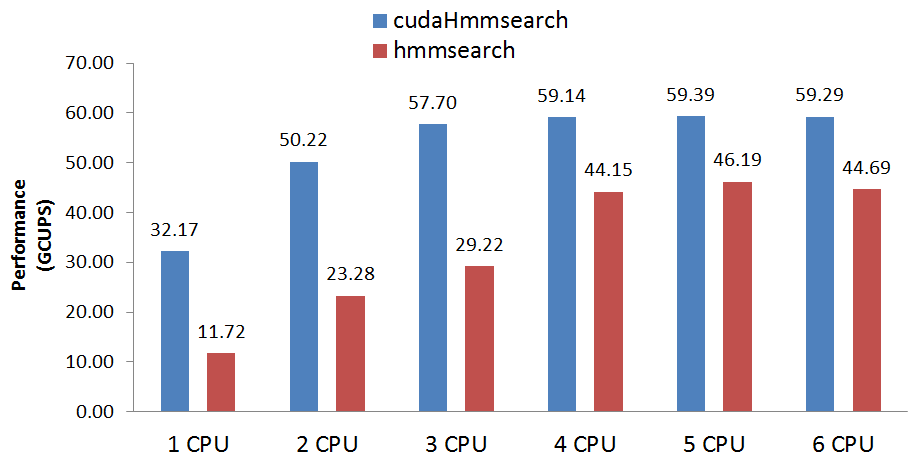
\includegraphics[totalheight=0.25\textheight]{Figures/cpuCores.png}
	\caption{\fontfamily{pag}\selectfont \textbf{Comparison with multicore CPU.} The data of this chart come from Table\ref{tab.mcpu}. The number on each bar is the Performance in GCUPS.}
	\label{fig:cpuCores}
\end{figure}

\subsection{Comparison with other implementations}
The performance of cudaHmmsearch was also compared to the previous HMMER solutions: HMMER2.3.2 \citep{HMMER2}, GPU-HMMER2.3.2 \citep{GPUHMM} and HMMER3 \citep{Hsource}.

All tests are taken searching against the Swiss-Prot database for the globin4 profile HMM.

\begin{table}[H]
\centering
\begin{tabular}{|c|c|c|c|c|}\hline
\shortstack{Application \\ (Device)} & \shortstack{HMMER2.3.2 \\ (CPU)} & \shortstack{GPU-HMMER2.3.2 \\ (GPU)} & \shortstack{HMMER3 \\ (CPU)} & \shortstack{cudaHmmsearch \\ (GPU)} \\\hline
\shortstack{Performance\\ (GCUPS)} & 0.14 & 0.95 & 8.47 & 17.36 \\\hline
\end{tabular}
\caption{\fontfamily{pag}\selectfont {Result of Comparison with other implementations.} \label{tab.hmms}}
\end{table}

As seen from the Figure\ref{fig:hmms}, since the release of HMMER2.3.2 in Oct 2003, accelerating hmmsearch researches on both CPU and GPU have achieved excellent improvement.

\begin{figure}[!htb]
	\centering
	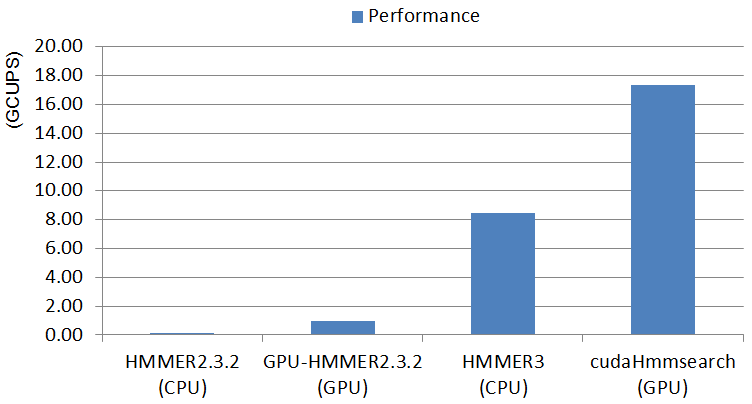
\includegraphics[totalheight=0.28\textheight]{Figures/manyhmms.png}
	\caption{\fontfamily{pag}\selectfont Comparison with other implementations.}
	\label{fig:hmms}
\end{figure}

%----------------------------------------------------------------------------------------

% Chapter 6

\chapter{Conclusions} % Main chapter title

\label{Conclusions} % For referencing the chapter elsewhere, use \ref{Chapter1} 

\lhead{Chapter 6. \emph{Conclusions}} % This is for the header on each page - perhaps a shortened title

A fully-featured and accelerated HMMER3 protein search tool \emph{cudaHmmsearch} was implemented on CUDA-enabled GPU. It can search the protein sequence database for profile HMMs.

%----------------------------------------------------------------------------------------

\section{Summary of Contributions}
Our research work started with dynamic programming, the common characteristic of Swith-Waterman algorithm, Viterbi algorithm and MSV algorithm, which are famous protein sequence alignment algorithms in Bioinformatics.
We specially summarized the technologies of accelerating Swith-Waterman algorithm on CUDA-enabled GPU, on which has been widely researched. We also briefly presented GPU acceleration work related to Viterbi algorithm.

After analyzing the core application \emph{hmmsearch} in HMMER3, we found the key hotspot MSV filter for accelerating hmmsearch. We presented the details of our \emph{cudaHmmsearch} implementation and optimization approaches. At the same time, we also discussed and analyzed the advantages and limitations of GPU hardware for CUDA parallel programming. Then we summarized 6 steps for better performance of CUDA programming.

We performed comprehensive benchmarks. The results were analyzed and the efficiency of the \emph{cudaHmmsearch} implementations on the GPUs is proved. We achieved 2.5x speedup over the single-threaded HMMER3 CPU SSE2 implementation. The performance analysis showed that GPUs are able to deal with intensive computations, but are very sensitive to random accesses to the global memory.

The solutions in this thesis were designed and customized for current GPUs, but we believe that the principles studied here will also apply to future manycore GPU processors, as long as the GPU is CUDA-enabled. Here is the complete list of CUDA-enabled GPUs: \url{https://developer.nvidia.com/cuda-gpus}.

%----------------------------------------------------------------------------------------

\section{Limitations of Work}
There are some weak points in our work summarized as follows:

Although our \emph{cudaHmmsearch} can search against unsorted protein sequence database, it can gain 129\% improvement searching against sorted database according to benchmark Table\ref{tab.opt}. And although the extra sorting database program is provided, user may be unaware of this and run \emph{cudaHmmsearch} against an unsorted database. It is better for the program to evaluate the database automatically and remind user to sort if necessary.

We use block reading method to process very large database. However, the number of sequences for each block reading is fixed. So the number of threads launched in GPU kernel is also fixed. For those sequences with shorter lengths, it is better to use dynamic block reading to get more sequences, so as to increase the occupancy of GPU threads and achieve better performance.

%----------------------------------------------------------------------------------------

\section{Recommendations for Future Research}
The limitations noted in the last section call attention to several areas that we deem worthy of further improvement and investigation. The suggested topics are placed under the following headings.

\subsection*{Forward filter for no threshold}
By default, the top-scoring of target sequences are expected to pass each filter. Alternatively, the -\emph{-max} option is available for those who want to make a search more sensitive to get maximum expected accuracy alignment. The option causes all filters except Forward/Backward algorithm to be bypassed. And according to practical benchmarking in Section\ref{Pbench}, the performance decreased greatly due to much more calculation in Forward algorithm. So our next research should be focused on accelerating Forward algorithm on CUDA-enabled GPU.

\subsection*{Multiple GPUs approach}
Since currently we don't have multiple GPUs within a single workstation, we didn't research on multiple GPUs approach. However, CUDA already provides specific facilities for multi-GPU programming, including threading models, peer-to-peer, dynamic parallelism and inter-GPU synchronization, etc. Almost all PCs support at least two PCI-E slots, allowing at least two GPU cards to insert almost any PC. Looking forward, we should also investigate multi-GPU solutions.

%----------------------------------------------------------------------------------------
 
%\input{Chapters/Chapter6} 
%\input{Chapters/Chapter7} 

%----------------------------------------------------------------------------------------
%	THESIS CONTENT - APPENDICES
%----------------------------------------------------------------------------------------

\addtocontents{toc}{\vspace{2em}} % Add a gap in the Contents, for aesthetics

\appendix % Cue to tell LaTeX that the following 'chapters' are Appendices

% Include the appendices of the thesis as separate files from the Appendices folder
% Uncomment the lines as you write the Appendices

% Appendix A

\chapter{Resource of this thesis} % Main appendix title

\label{AppendixA} % For referencing this appendix elsewhere, use \ref{AppendixA}

\lhead{Appendix A. \emph{Resource of this thesis}} % This is for the header on each page - perhaps a shortened title

The code of \emph{cudaHmmsearch} and this thesis has submitted to Google subversion server powered by Google Project Hosting and can be accessed in a web browser or subversion client with the address:
http://cudahmmsearch.googlecode.com/svn/trunk/
%\input{Appendices/AppendixB}
%\input{Appendices/AppendixC}

\addtocontents{toc}{\vspace{2em}} % Add a gap in the Contents, for aesthetics

\backmatter

%----------------------------------------------------------------------------------------
%	BIBLIOGRAPHY
%----------------------------------------------------------------------------------------

\label{Bibliography}

\lhead{\emph{Bibliography}} % Change the page header to say "Bibliography"

\bibliographystyle{unsrtnat} % Use the "unsrtnat" BibTeX style for formatting the Bibliography

\bibliography{Bibliography} % The references (bibliography) information are stored in the file named "Bibliography.bib"

\end{document}  